%%%%%%%%%%%%%%%%%%%%%%%%%%%%%%%
%This is the article LaTeX template for RSC journals
%Copyright The Royal Society of Chemistry 2010
%%%%%%%%%%%%%%%%%%%%%%%%%%%%%%%


\documentclass[8.5pt,twoside,twocolumn]{article}
\oddsidemargin -1.2cm
\evensidemargin -1.2cm
\textwidth 18cm
\headheight 1.0in
\topmargin -3.5cm
\textheight 22cm
\usepackage[super,sort&compress,comma]{natbib} 
\usepackage{mhchem}
\usepackage{times,mathptmx}
% \usepackage{times}
% feel free not to use mathptmx if it causes difficulties
\usepackage{sectsty}
\usepackage{balance} 

\usepackage{amsmath,graphicx} %eps figures can be used instead
\usepackage{lastpage}
\usepackage[format=plain,justification=raggedright,singlelinecheck=false,font=small,labelfont=bf,labelsep=space]{caption} 
\usepackage{fancyhdr}
\pagestyle{fancy}
%%%%%%%%%%%%%
\usepackage{graphicx}
\usepackage{etoolbox,hyperref}
\newcommand{\red}[1]{\textcolor{red}{#1}}
%%%%%%%%%%%%%%%%%%%
\begin{document}

\thispagestyle{plain}
\fancypagestyle{plain}{
\fancyhead[L]{\includegraphics[height=8pt]{headers/LH}}
\fancyhead[C]{\hspace{-1cm}\includegraphics[height=20pt]{headers/CH}}
\fancyhead[R]{\includegraphics[height=10pt]{headers/RH}\vspace{-0.2cm}}
\renewcommand{\headrulewidth}{1pt}}
\renewcommand{\thefootnote}{\fnsymbol{footnote}}
\renewcommand\footnoterule{\vspace*{1pt}% 
\hrule width 3.4in height 0.4pt \vspace*{5pt}} 
\setcounter{secnumdepth}{5}



\makeatletter 
\def\subsubsection{\@startsection{subsubsection}{3}{10pt}{-1.25ex plus -1ex minus -.1ex}{0ex plus 0ex}{\normalsize\bf}} 
\def\paragraph{\@startsection{paragraph}{4}{10pt}{-1.25ex plus -1ex minus -.1ex}{0ex plus 0ex}{\normalsize\textit}} 
\renewcommand\@biblabel[1]{#1}            
\renewcommand\@makefntext[1]% 
{\noindent\makebox[0pt][r]{\@thefnmark\,}#1}
\makeatother 
\renewcommand{\figurename}{\small{Fig.}~}
\sectionfont{\large}
\subsectionfont{\normalsize} 

\fancyfoot{}
\fancyfoot[LO,RE]{\vspace{-7pt}\includegraphics[height=9pt]{headers/LF}}
\fancyfoot[CO]{\vspace{-7.2pt}\hspace{12.2cm}\includegraphics{headers/RF}}
\fancyfoot[CE]{\vspace{-7.5pt}\hspace{-13.5cm}\includegraphics{headers/RF}}
\fancyfoot[RO]{\footnotesize{\sffamily{1--\pageref{LastPage} ~\textbar  \hspace{2pt}\thepage}}}
\fancyfoot[LE]{\footnotesize{\sffamily{\thepage~\textbar\hspace{3.45cm} 1--\pageref{LastPage}}}}
\fancyhead{}
\renewcommand{\headrulewidth}{1pt} 
\renewcommand{\footrulewidth}{1pt}
\setlength{\arrayrulewidth}{1pt}
\setlength{\columnsep}{6.5mm}
\setlength\bibsep{1pt}

\twocolumn[
  \begin{@twocolumnfalse}
\noindent\LARGE{\textbf{On scattered waves and lipid domains: detecting membrane rafts with x-rays and neutrons}}%\title{Scattering on lipid domains}
\vspace{0.6cm}

\noindent\large{\textbf{Drew Marquardt,\textit{$^{a,b}$} Frederick A. Heberle,\textit{$^{c,d}$} Jonathan D. Nickels,\textit{$^{c}$} Georg Pabst$^{\ast}$\textit{$^{a,b}$} and John Katsaras$^{\ast}$\textit{$^{c,d,e}$}}}\vspace{0.5cm}
%Please note that \ast indicates the corresponding author(s) but no footnote text is required. 


\noindent\textit{\small{\textbf{Received Xth XXXXXXXXXX 20XX, Accepted Xth XXXXXXXXX 20XX\newline
First published on the web Xth XXXXXXXXXX 200X}}}

\noindent \textbf{\small{DOI: 10.1039/b000000x}}
\vspace{0.6cm}
%Please do not change this text.

\noindent \normalsize{Understanding the physiological role of lipids in cell membranes is strictly coupled to determination of their impact on membrane structure using well-defined lipid-only model systems. Elastic and inelastic scattering experiments using neutrons or X-rays are non-invasive, probe-free techniques that provide such insight and have been advanced significantly in the past years. In particular recent developments allow to study details of structure, elasticity and interactions in phase-separated systems mimicking membrane rafts. We review the basic concepts underlying these developments.}
\vspace{0.5cm}
 \end{@twocolumnfalse}
  ]



%Footnotes
%\footnotetext{\dag~Electronic Supplementary Information (ESI) available: [details of any supplementary information available should be included here]. See DOI: 10.1039/b000000x/

%Please use \dag to cite the ESI in the main text of the article.
%If you article does not have ESI please remove the the \dag symbol from the title and the above footnotetext.

\footnotetext{\textit{$^{a}$~University of Graz, Institute of Molecular Biosciences, Biophysics Division, NAWI Graz, Humboldtstr. 50/III, Graz, Austria. Tel. +43 316 380 4989; E-Mail: georg.pabst@uni-graz.at}}
\footnotetext{\textit{$^{b}$~BioTechMed-Graz, Graz, Austria. }}
\footnotetext{\textit{$^{c}$~Oak Ridge National Laboratory, Oak Ridge, Tennessee 37831, United States. Tel: +1 865 274 8824; E-mail: katsarasj@ornl.gov}}
\footnotetext{\textit{$^{d}$~Joint Institute for Neutron Sciences, Oak Ridge, Tennessee 37831, United States.}}
\footnotetext{\textit{$^{e}$~Department of Physics, University of Tennessee, Knoxville, Tennessee 37996, United States.}}
\footnotetext{\textit{$^{f}$~Department of Physics, Brock University, St. Catharines, Ontario L2S 3A1, Canada.}}

%additional addresses can be cited as above using the lower-case letters, c, d, e... If all authors are from the same address, no letter is required

%\footnotetext{\ddag~Additional footnotes to the title and authors can be included \emph{e.g.}\ `Present address:' or `These authors contributed equally to this work' as above using the symbols: \ddag, \textsection, and \P. Please place the appropriate symbol next to the author's name and include a \texttt{\textbackslash footnotetext} entry in the the correct place in the list.}


\section{Introduction}

Biological membranes are complex, self-assembled composites of proteins, lipids and carbohydrates, whose hierarchical organization is fundamental to physiological processes. In particular, lateral organization of the lipid/protein layer of plasma membranes has attracted significant scientific interest, but also considerable controversy. The membrane raft paradigm invokes the existence of functional domains enriched in sphingolipids, cholesterol and specific proteins, such as glycophosphatidylinositol-anchored proteins, that facilitate diverse cellular signaling and transport processes~\cite{Lingwood.2010}. However, proof of  their existence in live cells has been elusive ~\cite{Kusumi.2012,Kraft.2013,Sevcsik.2015,Pan.2012}.

In contrast, domains are well-established in lipid-only model systems of plasma membranes~\cite{Feigenson.2009,Marsh.2009}. Such systems of reduced complexity allow for close scrutiny of the biophysical nature of lipid-lipid interactions and their potential in organizing lateral membrane structure. Over the years, a variety of experimental techniques have been applied to study the properties of lipid domains~\cite{Heberle.2014}. In this tutorial review we focus on the ability of x-rays and neutrons to interrogate the properties of lipid domains, using either elastic or inelastic scattering. The present work can be seen as a follow-up to one of our previous review articles~\cite{Pabst.2010}, which although summarized early scattering studies on lipid domains, it mainly focused on homogeneous lipid bilayers. Here we discuss progress in the field that has taken place over the past five years.

The review article is organized as follows. First, we give a brief introduction to lipid-only domains in model systems mimicking the plasma membrane. We then expand on the theory of elastic and inelastic scattering of lipid domains, and describe some illustrative examples. Finally, we conclude and give an outlook as to what can be expected in this area of research in the near future.

\section{Properties of Membrane Domains}

In multi-component mixtures, lipids minimize free energies arising from their chemical structure, leading to differences, for example, in membrane structure, hydrocarbon chain packing and chain order, and hydrogen bond formation, to name but a few. For example, in a binary mixture of lipids (e.g., A and B), these interactions can be parameterized by~\cite{Hill.1986}
\begin{equation}
	\omega_{AB} = g_{AB}-\frac{1}{2}\left( g_{AA}+g_{BB}\right),
\end{equation}
where $g_{AA}$, $g_{BB}$ and $g_{AB}$ are the interaction free energies between like (AA and BB) and unlike (AB) pairs. Typical values for $\omega_{AB}$ vary between $-1$ k$_B$T and $+0.7$ k$_B$T ~\cite{Almeida.2009}, where phase separation occurs for $\omega_{AB} > +0.55$ k$_B$T and random mixing for $\omega_{AB} = 0$~\cite{Heberle.2011}. Qualitatively, lipids prone to form gel phases (those with saturated acyl chains) and lipids prone to form fluid phases (unsaturated lipid species) will phase separate over a broad range of temperatures and compositions (reviewed by Marsh~\cite{Marsh.2009,Marsh.2010}).

When discussing lateral membrane heterogeneity, it is useful to distinguish between four cases: (i) random (ideal) mixing; (ii) non-random mixing or compositional fluctuations (i.e., “unstable domains”); (iii) nanoscopic domains; and (iv) macroscopic domains. Domain stability and size depends on the line tension $\gamma$, which defines the free energy of the domain boundary (see e.g. ~\cite{Kuzmin.2005}). That is, critical domain fluctuations occur at $\gamma = 0$. At small $\gamma$,  nanoscopic domains are formed, whereas at large $\gamma$ domains may grow to several microns in size. 

Figure~\ref{phase_diagram} shows a typical compositional phase diagram for raft-like ternary lipid mixtures of low-melting lipids (mainly di- or monounsaturated lipids), high-melting lipids (long chain disaturated phosphatidylcholines or sphingomyelin) and cholesterol. 

\begin{figure}
	\includegraphics[width=0.5\textwidth]{figures/phase_diagram.pdf}
	\caption{Generic compositional phase diagram for a ternary lipid mixture focusing on the temperature behavior of the L$_o$/L$_d$ coexistence regime. The dashed line indicates a tie-line, and the dashed-dotted line describes the critical transitions occurring at T$_c$. T$_m$ is the melting temperature. Other phase coexistence regions are not shown for purposes of clarity.}
	\label{phase_diagram}
\end{figure}



Cholesterol is highly abundant in mammalian plasma membranes, and is a very peculiar membrane lipid. Although weakly amphiphilic, it has a finite solubility in phospholipid membranes, beyond which it precipitates from the bilayer as cholesterol monohydrate crystals~\cite{Buboltz.1999}. In bilayers composed of saturated or monounsaturated chains, cholesterol's solubility limit depends strongly on the phospholipid headgroup, and can be understood in terms of the ``umbrella model'', where headgroups of neighboring lipids reorient to cover cholesterol's nonpolar surface, preventing its unfavorable exposure to water~\cite{JuyangHuang.1999}. The ability of different phospholipids to shield cholesterol should therefore depend, not only on headgroup size, but also on chain packing considerations. Indeed, a 3- to 4-fold reduction in cholesterol solubility has been found in highly unsaturated PC bilayers composed of arachidonoyl (C20:4) or docosahexaenoyl (C22:6) chains at both the \textit{sn}-1 and \textit{sn}-2 positions~\cite{StephenR.Wassall.2004}, and several studies have shown that cholesterol preferentially interacts with membrane lipids composed of disaturated acyl chains~\cite{Silvius.2003}.

In binary lipid mixtures, cholesterol is well-known for its ordering effect on the fluid lamellar phase (L$_\alpha$), leading to the liquid-disordered (L$_d$) and liquid-ordered (L$_o$) phases, at low and high cholesterol contents, respectively.  On the other hand, lamellar gel phases (L$_\beta$) are disordered by cholesterol~\cite{Mouritsen.1994}. (Note, that frequently L$_d$ is used synonymously with L$_\alpha$.) In describing the differences between these phases it is instructive to consider the two types of order that define the lamellar phases, namely translational or in-plane positional order (the spatial correlation between one lipid and another), and the chain configurational order of an individual lipid. These types of order are related to observables like the diffusion coefficient (translational order), hydrocarbon chain thickness and gauche/trans isomerization ratio (chain configurational order), all of which are are strongly coupled in the L$_\alpha$ and L$_\beta$ phases.  In other words, low translational order is accompanied by low configurational order (fluid phase), and \textit{vice versa} in the case of for gel phase bilayers. Cholesterol, however, has the unique property of decoupling these two types of order: the L$_o$ phase has very high chain order, but lacks long-range positional order. Properties of the lamellar phases are summarized in Fig.~\ref{phases}. 


\begin{figure}
\includegraphics[width=0.5\textwidth]{figures/phases.pdf}
\caption{Venn diagram of properties shared between the gel ($L_\beta$), liquid disordered ($L_d$) and liquid ordered ($L_o$) phases.}
\label{phases}
\end{figure}


In raft-like lipid mixtures, as shown in Fig.~\ref{phase_diagram}, L$_o$ and L$_d$ phases coexist over an extended range of compositions and temperatures. Since L$_o$ and L$_d$ are fluid phases, their $\gamma$ is isotropic, leading to the formation of circular domains. Demixing occurs along tielines, and L$_o$/L$_d$ composition can be read off the tieline endpoints, where they cross the phase coexistence boundary. The fraction of L$_o$ or L$_d$ changes along the tieline, and can be determined using the lever rule~\cite{Marsh.2009}. The direction of tielines may differ from system to system, but in general show that L$_d$ domains contain most of the low-melting lipid, whereas L$_o$ domains are enriched in the high-melting lipid and moderately enriched ($2$- to $3$-fold) in cholesterol.

At high temperatures, L$_o$ melts into a pure L$_d$ phase, giving the phase coexistence regime a dome-like structure. If this melting occurs at the peak of the ``dome'' it passes through a critical point $T_c$. Similarly, upon increasing cholesterol concentration, the L$_d$ phase melts into an L$_o$ phase. In this case, the tielines collapse into a single point, and the transition becomes second order. Thus, different critical transitions can be realized in ternary lipid mixtures, as shown in Fig.~\ref{phase_diagram}.

In the following section we describe how x-rays and neutrons can be used to probe domain size, namely static and dynamic domain structures. Understanding domain structure is needed for understanding how domains couple to protein partitioning and function. It is important to note that no bulky labels, which can potentially influence phase behavior~\cite{Ayuyan.2006,Zhao.2007,Veatch.2007}, are needed for the scattering studies described herein.

\section{General Scattering Theory}

Even though x-rays are electromagnetic waves and neutrons particle waves, a single scattering theory is used to address both types of experiments. However, there are some important differences that must be first considered. To begin, x-rays interact with electrons, while neutrons interact with the nuclei. Although not immediately obvious, x-ray scattering varies predictably with atomic number--heavy atoms scatter more strongly than lighter ones--while neutron scattering power varies erratically with atomic number. Importantly, however, is that neutrons are differentially sensitive to an element and its isotope(s). For example, hydrogen, which is ubiquitous in biological samples, has a coherent neutron scattering length $b_H^{coh} = -3.7423$ fm, while its stable isotope, deuterium, has $b_D^{coh} = 6.674$ fm. This difference between the two nuclei forms the basis of neutron contrast variation studies of biological materials. Therefore, by changing either the external contrast (by varying the H$_2$O/D$_2$O composition of the aqueous buffer), or by selectively deuterating specific parts of the biomolecule of interest~\cite{Fitter.2006}, one can highlight or suppress static and dynamic structural features. 

Another important difference between x-rays and neutrons scattering relates to instrumental resolution. The wavelength spread $\Delta \lambda/\lambda$  at third generation synchrotron small-angle x-ray scattering (SAXS) beamlines is of the order of 0.01\%, approximately 2 orders of magnitude tighter than what is encountered at neutron beamlines. The main reason for this difference is the relatively low flux of neutron instruments, compared to x-rays, requiring monochromators capable of accepting broader range of neutron wavelengths (i.e., less monochromatic beams). An obvious consequence of this, is that SAXS peaks are significantly sharper than peaks from small-angle neutron scattering (SANS) instruments. This offers the possibility to perform line-shape analysis, resulting in the bilayer's elastic constant (see below). A less obvious result of tighter collimation and increased monochromicity relates to the beam coherence volume $V_{coh}$, which is described in terms of partial coherence in the theory for optics ~\cite{Born.1980}. $V_{coh}$ has a longitudinal component, i.e. parallel to the propagating wave train, 
\begin{equation}
L_{coh} = \frac{\lambda^2}{\Delta \lambda} = \frac{2 E}{\Delta E} \lambda,
\end{equation}
where $\Delta E/E$ is the energy resolution of either the neutron or x-ray beam, and two transverse components $T_{coh}^{i}$ which vary inversely with the source aperture size~\cite{Bernhoef.1998, Felber.1998}. Typical values for $L_{coh}^{x-ray}$ at synchrotron beamlines are on the order of 1 $\mu$m, while $L_{coh}^{neutron} \le 0.05$ $\mu$m. The coherence volume is of particular importance when detecting membrane domains, as will be discussed later on. 


There is a third important difference between neutrons and x-rays. Neutron energies are typically on the order of meV, which are well within the range of thermally excited molecular motions, while x-rays are usually on the order of keV. Thus, while coherent inelastic x-ray scattering experiments on lipid membranes are feasible~\cite{Chen.2001,Weiss.2003}, neutrons are better suited~\cite{Rheinstadter.2006}. 


\subsection{Elastic X-ray and Neutron Scattering}

In the case of elastic scattering there is no transfer of energy. It is therefore sufficient to consider the change in scattered intensity as a function of the wave vector transfer, $q$. The vector \textbf{q} is proportional to the angle between the incoming and outgoing beams (i.e., the scattering angle, $2\theta$). The scattering vector, $q$, is then given by $q=4\pi\sin(\theta)/\lambda$, where $\lambda$ is the x-ray or neutron wavelength. Coherent elastic scattering of neutrons or X-rays provides information regarding spatial correlations of nuclei or electrons, respectively. However, unlike in a crystal, where atoms are restricted to small thermal vibrations around well-defined positions, the inherent disorder of fluid lipid membranes prevents structure determination at atomic resolution. Thus it has proven useful to sum up the electrons or neutron scattering lengths per unit volume, and introduce the concept of the electron density profile (EDP) or neutron scattering length density (NSLD) profile (see sec.~\ref{sec:sdp}).

Spatial correlations are contained in the amplitudes of the scattered wave or form factor F($\bf{q}$). F($\bf{q}$) is the sum of the coherent scattering length ($b^{coh}$) of all atoms in the sample (Eq.~\ref{fq}), and is proportional to the observed intensity of the scattered wave (Eq.~\ref{Iq}).



\begin{equation}
\label{fq}
F({\bf{q}}) = \sum_{i}^{atoms} b^{coh}_i e^{i{\bf{q}}\cdot r_i}
\end{equation}



\begin{equation}
I({\bf{q}}) \propto |F({\bf{q}})|^2 S_p({\bf{q}})
\label{Iq}
\end{equation}



The real-space distribution of the scattering lengths (the scattering length density, $\rho$) is the Fourier transform of the form factor, 
%
\begin{equation}
\label{SLD}
\rho(r) = \int F({\bf{q}}) e^{-i{\bf{q}}\cdot r} d{\bf{q}} \space
\end{equation}
%
From the real-space distribution of $\rho$, membrane structural parameters can be determined as discussed in sec. \ref{sec:sdp}.

%Because only the intensities of the scattered waves can be measured and not the phase shifts, a direct transformation back into real space is usually inhibited.


The second term in I($\bf{q}$) is the inter-particle structure factor $S_p(\bf{q})$ describing the relative positions of particles, which can be formulated by a variety of theories~\cite{Klein.2002} and is often approximated by $S_p(\bf{q}) = 1$ for dilute systems. Positional correlations in multibilayer systems give rise to an additional structure factor $S_i(\bf{q})$ accounting for interactions between the sheets that give rise to long-range order, and hence the Bragg peaks. In the case of lipid multibilayers in the fluid L$_\alpha$ phase, true long-range order breaks down due to pronounced bilayer bending fluctuations resulting in \textit{quasi} long-range order--power law decay describing positional correlations~\cite{Jeu.2003}. This leads to a characteristic cusp-like peak shape that can be described by Caill\'{e} theory~\cite{Caille.1972,Zhang.1994}. For multilamellar vesicles (MLVs) the structure factor is given by~\cite{Pabst.2000}
%
\begin{equation}
\label{eq:caille}
	S_i(q)=N+2\sum_{k=1}^{N-1} (N-k) \cos(k q d) e^{-(d/2\pi)^2 \eta \left[\gamma + \ln (\pi k)\right]},
\end{equation}
%
where $N$ is the number of layers per scattering domain, $d$ the lamellar repeat distance, and $\gamma$ is Euler's constant. (We note that the modulus of the scattering vector $q$ can be used due to orientational averaging in MLVs.) Of particular importance is the Caill\'{e} or fluctuation parameter,
%
\begin{equation}
\label{eq:eta}
	\eta = \frac{\pi k_B T}{2 d^2 \sqrt{B K_c}}
\end{equation}
which is a function of the bulk modulus of compression $B$ and the bilayer bending rigidity~\cite{Zhang.1994} ($k_B$ is Boltzmann's constant and $T$ temperature).




\subsection{Inelastic Scattering}\label{InES}
%\textbf{Jonathan, please fill in here...}
In contrast to the elastic scattering experiments described above, inelastic scattering approaches are defined by the transfer of energy and momentum between the incident and outgoing beams.  The inelastic scattering of neutrons is ideal for studies of molecular motion in lipid bilayers--though its potential is relatively unexploited to date. The incident energy of neutrons typically used in inelastic scattering experiments is, as mentioned, on the order of meV and comparable to the time regimes commonly observed in many processes taking place in soft materials, such as diffusion, vibrations, methyl rotation and other molecular reorientations, lipid rotation, bilayer undulation, and bilayer thickness fluctuations. The goal of inelastic scattering experiments is to measure two quantities, namely the momentum transfer, $q= k_f-k_i$, and the energy transfer, $\hbar\omega=E_f-E_i$.  Here, $k_i$ and $k_f$ are the wave vectors, and $E_i$ and $E_f$ are the energies of the incident and scattered neutrons, respectively. Through these two quantities, one can extract detailed information with respect to the frequency and geometry of atomic motions within a lipid bilayer, and between it and its local environment.  

The earliest inelastic scattering experiments were performed in the 1950s by Bertram Brockhouse~\cite{Brockhouse.1955} at the then Chalk River Nuclear Laboratories using his newly developed triple-axis spectrometer.  This novel way of measuring inelastic scattering enabled the measurement of scattered intensity at specific points in $q$ and $\omega$. However, this approach is not convenient for studies of lipid bilayers. A range of specialized spectrometers have subsequently been designed to optimize observation of scattered intensity simultaneously at multiple points in phase space, including time-of-flight ~\cite{Copley.1993}, backscattering~\cite{Maier.1966} and neutron-spin-echo (NSE) spectrometers~\cite{Mezei.1972}. This modern suite of instruments is able to probe motions on timescales ranging from $10^{-14}$~s to $10^{-7}$~s, and over length scales from $10^{-7}$~m to less than $10^{-10}$~m.

A quantitative description of inelastic scattering~\cite{VanHove.1954,Bee.1988,Gennes.1963} requires us to consider the basic quantity measured by neutron scattering experiments, namely the double differential cross-section, which can be written as follows: 

\begin{equation}
\label{eq:Jon1}
\frac{\partial ^2 \sigma}{\partial \Omega \partial \omega} = \frac{k_f}{k_i} \left((\langle b^2 \rangle - \langle b \rangle ^2) S_{inc}(q,\omega) + \langle b \rangle ^2 S_{coh}(q,\omega) \right)  
\end{equation}


When this quantity is multiplied by the number of incident neutrons, it ends up describing  the number of neutrons scattered into a solid angle element $\partial\Omega$ with an energy transfer $\hbar\omega$. The variable $b$ describes the scatting length of the sample, and $S(q,\omega)$ is the dynamic structure factor. This relation brings to the fore the other major difference between neutron and X-ray scattering, specifically the presence of both incoherent, $S_{inc}(q,\omega)$ and coherent, $S_{coh}(q,\omega)$ scattering in the case of neutrons. 

Separate dynamic structure factors, $S_{coh}(q,\omega)$ and $S_{inc}(q,\omega)$, describe these two classes of scattering. Each is connected to the microscopic motions of the atoms in the sample, but in different ways. Coherent scattering is related to the double Fourier transform in space and time of the density-density correlation function.  This is typically expressed in terms of atom positions, $r_j$ and $r_i$ at time, t, and time, 0 as follows:

\begin{equation}
\label{eq:Jon2}
S_{coh}(q,\omega)=\frac{1}{2\pi N}\int dt \langle \sum_{i,j} e^{i(q\left(\cdot r_j(t)-r_i(0) \right)-\omega t)}\rangle
\end{equation}

As a result, $S_{coh}(q,\omega)$ is interpreted as a representation of the probability of finding an atom at time, $t$, at a distance, $r$, from another atom at time 0. On the other hand, the incoherent scattering function, $S_{inc}(q,\omega)$, reflects the probability of finding an atom at a time, $t$, within a distance, $r$, from its initial position at time 0. Explicitly this is the double Fourier transform in space and time of the self-correlation function: 

\begin{equation}
\label{eq:Jon3}
S_{inc}(q,\omega)=\frac{1}{2\pi N}\int dt \langle \sum_{i,j} e^{i(q \cdot \Delta r_i(t) -\omega t)}\rangle
\end{equation}


This relates the scattering to motions of individual atoms, and is thus more straightforward to interpret than $S_{coh}(q,\omega)$, especially in the case of single potential well motions. (This is a special case where a mean square displacement can be directly extracted~\cite{Zaccai.2000} from the elastic intensity for a given temporal instrumental resolution.)  

The most common type of inelastic scattering measurement for biological materials focuses on the incoherent scattering from hydrogen. Hydrogen ($^1$H) has an incoherent scattering cross-section of 80.27 barns, 40 times greater than $^2$H, and more than 100 times larger than the other elements in lipid bilayers: C ($\sim$0.001 barns); N (0.5 barns); O (0.0008 barns); and P (0.005 barns). Because of this high incoherent scattering from hydrogen, incoherent scattering experiments often use hydrogenated or partially deuterated lipids, hydrated with D$_2$O in order to isolate the scattered signal from the lipid component of interest within the sample~\cite{Pfeiffer.1989,Wood.2008,Armstrong.2010,Konig.1992,Rheinstadter.2012,Rheinstadter.2005,Swenson.2008,Fitter.1999}. Naturally, this situation can be reversed to study the dynamics of hydration water using a deuterated bilayer~\cite{Swenson.2008,Konig.1994,Nickels.2012}.

The scattered intensity is customarily reduced to a function of $\omega$ for a set of $q$ values. Analysis of inelastic incoherent scattering data yields information about the geometry and relaxation times of atomic motions within the sample~\cite{Vineyard.1958}). The geometric information for a given dynamic process is usually extracted from the ratio of elastic intensity to total scattered intensity, and is represented as a phenomenological quantity called the Elastic Incoherent Structure Factor or $EISF(q,\omega)$. Numerous functional forms of the $EISF$ have been put forward in order to accurately model the various atomic motions probed by scattering experiments~\cite{Fitter.1996}. The inelastic scattering term is modeled with a Lorentzian function $\Gamma(q,\omega)$ that results in a relaxation time as a function of $q$. When the inelastic contribution of each process is combined with the $EISF$, and a delta function, $\delta(\omega)$, to account for elastic scattering, this then allows us to write the theoretical scattering function,  


\begin{eqnarray}
\label{eq:Jon4}
S_{Theo}(q,\omega)= \sum_{i=1}^{n} P_i(EISF_i(q,\omega)\delta(\omega) + \nonumber \\ 
\left[(1-EISF_i(q,\omega)) \ast \Gamma_i(q,\omega) \right]
\end{eqnarray}

which can be fit against experimental data,

\begin{equation}
\label{eq:Jon5}
S_{Exp}(q,\omega)= DWF(q) \ast \left[ S_{Theo}(q,\omega) \otimes R(q,\omega) \right]
\end{equation}

Here, $DWF(q)$ represents the Debye-Waller Factor and $R(q, \omega)$ is the instrumental resolution function that defines the time and length scales probed by the experiment, and is an important consideration for both the design of the experiment and analysis of the data~\cite{Nickels.2012b}. 

Deuterated molecules are also used to study inelastic coherent scattering by reducing the overwhelming incoherent signal from hydrogen. This class of experiment excels in studies of lattice dynamics~\cite{Copley.1974,Nielsen.1973}, but can also be useful in the study of collective motions of soft matter~\cite{Buchenau.1986,Carpenter.1985,Nickels.2013,Neumann.1991,Rheinstadter.2004}. Treatment of coherent scattering data is somewhat more complicated due to sensitivity to pair-correlations. On the other hand, this sensitivity leads to the key feature of inelastic coherent scattering measurements, namely the ability to observe which atomic spacings are preserved during a particular collective motion. This information can be accessed by plotting the scattered intensity as a function of $q$, for a set of $\omega$s, and comparing to the static structure factor, $S(q,0)$. When a set of atoms move collectively, maintaining their relative spacing, they will give rise to excess intensity written as follows: 

\begin{equation}
\label{eq:Jon6}
S(q,\omega)= A(\omega) \ast  S(q,0) \ast q^2 + B(\omega) \ast q^2 + C 
\end{equation}

Here the first term represents the excess scattering from pair correlations that are preserved during a motion at a given $\omega$, the second term represents incoherent and out of phase motions, which follow a $q^2$ dependence, and the third term covers any $q$ independent multiple scattering. This relation does not hold for atomic spacings in $S(q,0)$ which are violated during a particular motion, clearly illustrating which atom pairs are moving together and which are not. 

The NSE technique is different in terms of data analysis. The primary distinction of NSE, compared to the other inelastic techniques, is that it measures the intermediate scattering function, ISF or $I(q,t)$, rather than the dynamic structure factor, $S(q,\omega)$. It is typically reported as $I(q,t)/I(q,0)$ so that the quantity is normalized to 1. $I(q,t)$ is simply the Fourier transform of the dynamic structure factor in the time domain.  The other difference is that fitting of the data is typically performed in the time domain, so rather than using peak functions to fit the data, decay functions are used instead. Although NSE is capable of probing slow diffusive motions of lipids and fluctuations of bilayer thickness, the most common spin-echo experiments on lipid bilayers are direct measurements of bilayer undulation, enabling one to access the bilayer's bending modulus~\cite{Woodka.2012,Arriaga.2010,Pan.2015,Yi.2009,Lee.2010,Nickels.2015}. Observations of the coherent scattering from the bilayer in the range of 0.05 to 0.2 \AA$^{-1}$ are made and data are analyzed using a modified~\cite{Woodka.2012,Lee.2010,Watson.2010} Zilman and Granek analysis~\cite{Zilman.1996}. In the time domain, the first step is to fit the ISF using the following relation: 

\begin{equation}
\label{eq:Jon7}
\frac{I(q,t)}{I(q,0)} = A e^{-(\Gamma(q)\cdot t)^{\frac{2}{3}}}
\end{equation}

Here a stretched exponential decay is used with, $A$, as a normalization constant (typically set to 1) and $\Gamma(q)$ as the relaxation rate, which is a function of the scattering wave vector, $q$. The relaxation rate is related to the bilayer bending modulus $\kappa$ through, 

\begin{equation}
\label{eq:Jon8}
\Gamma(q) = 0.0058 \left( \frac{k_BT}{\kappa}\right)^{\frac{1}{2}} \frac{k_B T}{\eta}q^3
\end{equation}

where, $\eta$, is the solvent viscosity, $k_B$ is Boltzmann’s constant, and $T$ is the temperature. This relation implies that a plot of $\Gamma(q)/q^3$ as a function of $q$ will exhibit a constant value that is inversely proportional to the square root of the bending modulus. 

\section{Sample Geometries}
As discussed, lipid domains can be studied using a variety of scattering techniques, however, some of which demand unique sample preparations, conditions and geometries. From the standpoint of biological relevance, unilamellar vesicles (ULVs) are the most desirable mimics of a cellular membrane. Diffuse scattering from a dilute ULV suspension affords the possibility to extract the bilayer's continuous F($\bf{q}$) (Eqn.~\ref{Iq}), and often offers extended ranges for the scattering vector's transverse component ($\bf{q}_z$).

Arguably the easiest method of sample preparation is that of MLVs, whereby a dry lipid mixture film is hydrated with water. Measurement of MLVs results in the presence of a $F(\bf{q})$ and a $S_i(\bf{q})$ as a  convolution of both the radial and in-plane heterogeneities of the bilayer structure. A great deal of information can be extracted from MLV samples, including (but not limited to) the ``stiffness'' of the bilayer and the presence of domains (sec.~\ref{sec:phase_sep}).

Supported samples can be generated as a single bilayer typically examined with reflectometry, or as multilamellar stacks interrogated by diffraction techniques. Although MLV samples are aligned bilayers, alignment on a solid substrate allows for the transverse and lateral structures to be examined independently. The separation of ${\bf{q}}_z$ and ${\bf{q}}_{||}$ (the lateral scattering vector component) allows for the unambiguous assignment of scattering features arising from the different orientations. Like all systems, solid-supported bilayers suffer from some drawbacks. Supported lipid bilayers have proven difficult to fully hydrate (Katsaras 1997 and 1998 BJ REFERENCES), though recent advances in sample environments have achieved hydration levels of better than 99.6\% as determined by the lamellar repeat spacing~\cite{Armstrong.2013}. The effects attributed to bilayer--substrate interactions are limited to the first few bilayers, although much effort has been expended into functionalizing the substrate surface with a polymer cushion for use in single bilayer studies~\cite{Naumann.2002}.

%*********************************
\begin{figure}
	\centering
	\includegraphics[width=0.45\textwidth]{figures/geometries3.png}
	\caption{Schematic diagram of an aligned bilayer setup. $\textbf{a}$) A ``white'' beam of incident radiation, $\textbf{b}$) monochromator selects a single wavelength of neutrons or X-rays. $|$k$_i$$|$ is the incident vector of monochromatic beam and $|$k$_s$$|$ is the scattered wave vector of same energy ($|$k$_i$$|$=$|$k$_s$$|$)--the case for elastic scattering. $\textbf{c}$) is the model membrane sample oriented such that the scattering vector (q$_z$) is perpendicular to the bilayer surface and $\textbf{d}$) is the detector. The lower schematic has the same spectrometer setup, the only difference is $\bf{e}$),where the bilayer is oriented such that the scattering vector (q$_{||}$) is parallel to the bilayer surface}
	\label{geo}
\end{figure}
%***********************************


The aforementioned sample conditions are characterized by low-resolution data, however, improved structural data can be achieved by utilizing the neutron scattering method of contrast variation.
% * <fred.heberle@gmail.com> 2015-07-02T15:49:01.143Z:
% what does "characterized by low-solution data" mean?
One clear advantage elastic neutron scattering has over other biophysical techniques, including X-ray scattering, is the ability to change contrast conditions without resorting to bulky and unnatural probes that can alter the bilayer's physical properties~\cite{Marquardt.2014}. The ability to manipulate contrast is particularly important since the scattering intensity is proportional to the square of the SLD difference between the sample and solvent (medium).
Contrast can be systematically manipulated by substituting one isotope of an element with another(discussed previously). In the case of biological samples, the substitution of hydrogen for deuterium is commonly used to manipulate contrast, as shown in Figure \ref{contrast}~\cite{T.A.Harroun.2006}. Scattering from individual components of the system, such as phase separated regions of a vesicle, can be suppressed through contrast matching with the solvent, allowing for the determination of \emph{lateral structure} and composition. Discussion of contrast variation in a SANS experiment is discussed below (Section \ref{SANS_domains}).

%*********************************
\begin{figure}
	\centering
	\includegraphics[width=0.45\textwidth]{figures/contrast}
	\caption{Schematic of possible neutron contrast variation experiments for a~ lipid bilayer. $\bf{A}$ represents the system with minimal contrast matching. $\bf{B}$) Contrast between lipid species can be generated by substituting the protiated species (grey) with a deuterated analogue (pink). $\bf{C}$) Matching the solvent to a one lipid species, rendering it ``silent''.}
	\label{contrast}
\end{figure}
%***********************************

\section{Homogeneously mixed bilayers: a brief update}
\label{sec:sdp}
Although homogeneously mixed fluid bilayers lack long range in-plane atomic correlations, they do possess one-dimensional out-of-plane correlations. The structure of a homogeneous fluid bilayer can therefore be thought of as the time-averaged distribution of matter projected onto the bilayer normal. A scattering experiment provides a distorted reflection of this matter distribution, where similar to a distorted mirror, features are reshaped by the relative interaction strength of the probe (neutrons or X-rays) with the lipid's chemical makeup. In this sense, the real-space scattering length density profiles obtained from different types of scattering experiments (i.e., X-ray data, or different contrast neutron data) are simply different representations of the bilayer's structure.  While traditional bilayer structural analyses models SLD profiles of standalone scattering data~\cite{Pabst.2000,Kucerka.2004,Kiselev.2006,Pencer.2006,Brzustowicz.2005,OliveiraCristianoL.P..2012}, a model based on matter density distribution can easily combine differently contrast  data sets (i.e., X-ray and neutron) into a single global analysis, resulting in a more robust structure of the bilayer. 

White and coworkers were the first to exploit this fundamental link between the bilayer's different chemical moieties, in their development of the so-called composition space model". Because individual atoms are not well-localized in a thermally disordered bilayer, they are best described by broad statistical averages. King and White~\cite{King.1986} proposed a coarse-grained lipid structure, where neighboring atoms are grouped into quasi-molecular distributions whose atomic number density profiles are described by simple functional forms (e.g., uniform or Gaussian distributions). A fully resolved fluid bilayer structure consists of a handful of such quasi-molecular distributions, typically 2-3 such distributions are used to describe the lipid headgroup, while 3-4 distributions are used for the hydrocarbon chain region. Scattering length density profiles for different contrast data sets are then obtained by scaling the component number density distributions with an appropriate scattering length (i.e., the sum of individual atomic scattering lengths making up the distribution). Through the joint refinement of neutron and X-ray diffraction data, Wiener and White determined the fully resolved structure of a partially dehydrated fluid DOPC bilayer~\cite{Wiener.1991,Wiener.1991b,Wiener.1991c,Wiener.1992,Wiener.1992b}.

Ku\v{c}erka et al.~extended this approach with their Scattering Density Profile (SDP) analysis (Fig.~\ref{fig:SDP_model}), which leverages the atomistic detail of MD simulations to guide the choice of atomic groupings, thereby maximizing the model's compatibility with different contrast X-ray and neutron data~\cite{Kucerka.2008}. For this model, which uses ULVs, Eq.~(\ref{fq}) becomes 
\begin{equation}
	\label{eq:SDP_formfac}
	F(q) = 2 \int_{0}^{d} \Delta \rho(z) e^{-i q z} dz,
\end{equation}
with
\begin{equation}
	\Delta \rho(z)= \sum_{i}^{n} (\rho_i - \rho_W) P_i(z).
\end{equation}
%
Here $P_i(z)$ represent the volume distribution functions of given molecular fragments, each described by a Gaussian or error function. A typical parsing scheme for a phosphatidylcholine bilayer would be, for example, the choline methyl (CholCH$_3$), phosphate + CH$_2$N (PCN), carbonyl + glycerol (CG), hydrocarbon methylene (CH$_2$) and terminal acyl chain methyl (CH$_3$) groups. The $P_i$'s are scaled by the contrast of their given scattering length densities $\rho_i$ to water $\rho_W = 0.33$ e/\AA$^3$ (X-rays)/ $\rho_W = -5.6 \times 10^{-7}$~\AA$^{-2}$ (neutrons).
\begin{figure}
	\centering
	\includegraphics[width=0.45\textwidth]{figures/SDP_scheme}
	\caption{Description of membrane structure in terms of the SDP model. Panel A shows a schematic of a stack of membranes with the corresponding structural parameters: $d$\ldots lamellar repeat distance; $d_B$\ldots bilayer thickness; $d_W$\ldots bilayer separation; $d_C$\ldots hydrocarbon chain length; $d_{HH}$\ldots headgroup-to-headgroup distance; and $A$\ldots area per lipid. Panel B shows the volume distribution functions of quasimolecular distributions  in term of the SDP model. Figure adapted from~\cite{Kucerka.2011}.}
	\label{fig:SDP_model}
\end{figure}

By combining SANS data at several D$_2$O/H$_2$O ratios (``external'' contrasts) with SAXS data, the authors obtained the first fully resolved bilayer structure from a vesicle suspension at full hydration. The SDP approach has since been used to determine structures for a wide range of biologically relevant lipids using fully hydrated fluid bilayers, including phosphatidylcholine~\cite{Kucerka.2009,Kucerka.2011}, phosphatidylglycerol~\cite{Pan.2014b}, phosphatidylserine~\cite{Pan.2014}, phosphatidylethanolamine~\cite{Kucerka.2015}, and cardiolipin~\cite{Pan.2015}. A major achievement of the SDP model is the robust determination of bilayer thickness, defined as
%
\begin{equation}
	d_B = d - 2\int_{0}^{d/2} P_W(z) dz,
\end{equation}
%
and area per lipid  
%
\begin{equation}
	A = \frac{2 V_L}{d_B},
\end{equation}
%
quantities that are crucial for the validation of MD force fields (reviewed in~\cite{Heberle.2012}). Here, $d$ is the lamellar repeat distance, $P_W$ the volume distribution function of water, and $V_L$ the lipid's molecular volume, which is obtained by separate experiments.

Recently, Heftberger et al.~\cite{Heftberger.2014} combined the SDP model with a Caill\'{e} structure factor (Eq.~\ref{eq:caille}), allowing them to analyze MLVs in the L$_\alpha$ phase (Fig.~\ref{fig:SDP_MLV}). In this case, the scattered intensity is given by
\begin{equation}
\label{eq:SDP_GAP}
	I(q) \propto \frac{|F(q)|^2}{q^2}\left[(1-N_{diff}) S_i(q) + N_{diff} \right],
\end{equation}
where $F(q)$ is given by Eq.~(\ref{eq:SDP_formfac}) and $S_i(q)$ by Eq.~(\ref{eq:caille})--the scalar $N_{diff}$ accounts for the presence of positionally uncorrelated bilayers. An advantage of this hybrid model is that membrane structure can be studied at SDP resolution without the need of extruded ULVs.  Further, by using the structure factor an experimental window on membrane fluctuations (Eq.~\ref{eq:eta}) becomes accessible, opening new opportunities to study bilayer interactions and membrane mechanical properties (see sec.~\ref{sec:elatic_xray}).

\begin{figure}[t]
	\centering
	\includegraphics[width=0.4\textwidth]{figures/SDP_MLV}
	\caption{Joint analysis of SAXS (inset) and SANS data of POPC MLVs and ULVs. Panel A shows SANS data of POPC (circles) and chain deutrated POPC-d31 (triangles) MLVs. Panel B shows corresponding data for ULVs (same symbols). Figure is adapted from~\cite{Heftberger.2014}.}
	\label{fig:SDP_MLV}
\end{figure}


\section{Phase separated bilayers}
\label{sec:phase_sep}

The importance of coherence volume $V_{coh}$ was discussed for phase separated systems. In particular, the dimensions of the domain size, or more precisely, the domain volume $V_D$ with respect to $V_{coh}$ need to be considered. If $V_{coh} \ge V_D$ scattering contributions of domains add up coherently, that is for ULVs exhibiting two-phase coexistence, then
\begin{equation}
	I(q) \propto | \phi_A F_A + (1-\phi_A) F_B|^2,
\end{equation}
where $\phi_A$ is the fraction of phase $A$, and $F_A$ and $F_B$ are the form factors of phases $A$ and $B$, respectively. If in turn $V_{coh} < V_D$, the form factors add up incoherently. Thus, for the same phase separated system we now get
\begin{equation}
I(q) \propto \phi_A |F_A|^2 + (1-\phi_A) |F_B|^2 + \tilde{I}(q),
\end{equation}
where $\tilde{I}(q)$ accounts for the coherent addition of form factors in the domain boundary regime, and where both phases exist within single $V_{coh}$ element. The latter contribution is typically neglected in the analysis of transverse domain structure~\cite{Heftberger.2015}. Note also that both equations assume an infinitesimally sharp domain boundary, which if it were not the case would result in an additional contribution.


The effect of $V_{coh}$ has been demonstrated by Armstrong et al.~\citealp{Armstrong.2012b} on single-component dipalmitoyl phosphatidylcholine (DPPC) in the vicinity of the main-phase transition regime. Cooling from the liquid disordered L${\alpha}$ phase, small gel-like domains begin to nucleate. Using neutron diffraction and oriented multibilayers, and by selectively detuning the pyrolytic graphite monochromator, Armstrong and co-workers were able to  decrease $L_{coh}$ from  $242$ \AA\/ to $30$ \AA. Only for $L_{coh} \le 103$ \AA\/ was phase coexistence observed.

With regard to domain size, another factor to consider is the overall ULV size. For 50 - 100 nm diameter ULVs, as studied by SANS (see section \ref{SANS_domains}), $V_{coh} > V_D$ for L$_o$/L$_d$ phase coexistence, allowing for domains to be detected (see sec.~\ref{SANS_domains}). In multibilayers, domains may grow up to several microns. In such cases, $V_{coh} < V_D$. This gives rise to two lamellar lattices from which one can measure each domain's transverse structure (see sec.~\ref{sec:elatic_xray}). However, things may differ for lipid mixtures exhibiting nanoscopic domains~\cite{Heberle.2013}, where domain size is of the order of $V_{coh}$. 

\subsection{Elastic neutron scattering - SANS}
\label{SANS_domains}
%*******************Fred's*******************************
\subsubsection{Detecting domains. }
As discussed in Section 5, the combination of SAXS and SANS provides detailed  information about the distribution of matter in the direction of the bilayer normal, allowing for the robust determination of lipid areas and thicknesses in homogeneous bilayers. Such studies rely on SLD differences between the solvent and bilayer--for SANS, a typical experiment uses fully protiated lipids in 100\% D$_2$O. Though optimal for studying transverse bilayer structure, these conditions largely mask the scattering signatures of lateral phase separation. As shown schematically in the upper panel of Fig. \ref{fig:SANS_domains}, a large solvent/bilayer contrast easily overwhelms any contrast generated by lipid segregation within the bilayer plane. Clearly, standard experimental conditions must be modified to suppress scattering arising from transverse contrast, and enhance scattering arising from lateral contrast.


\begin{figure} [t]
	\centering
	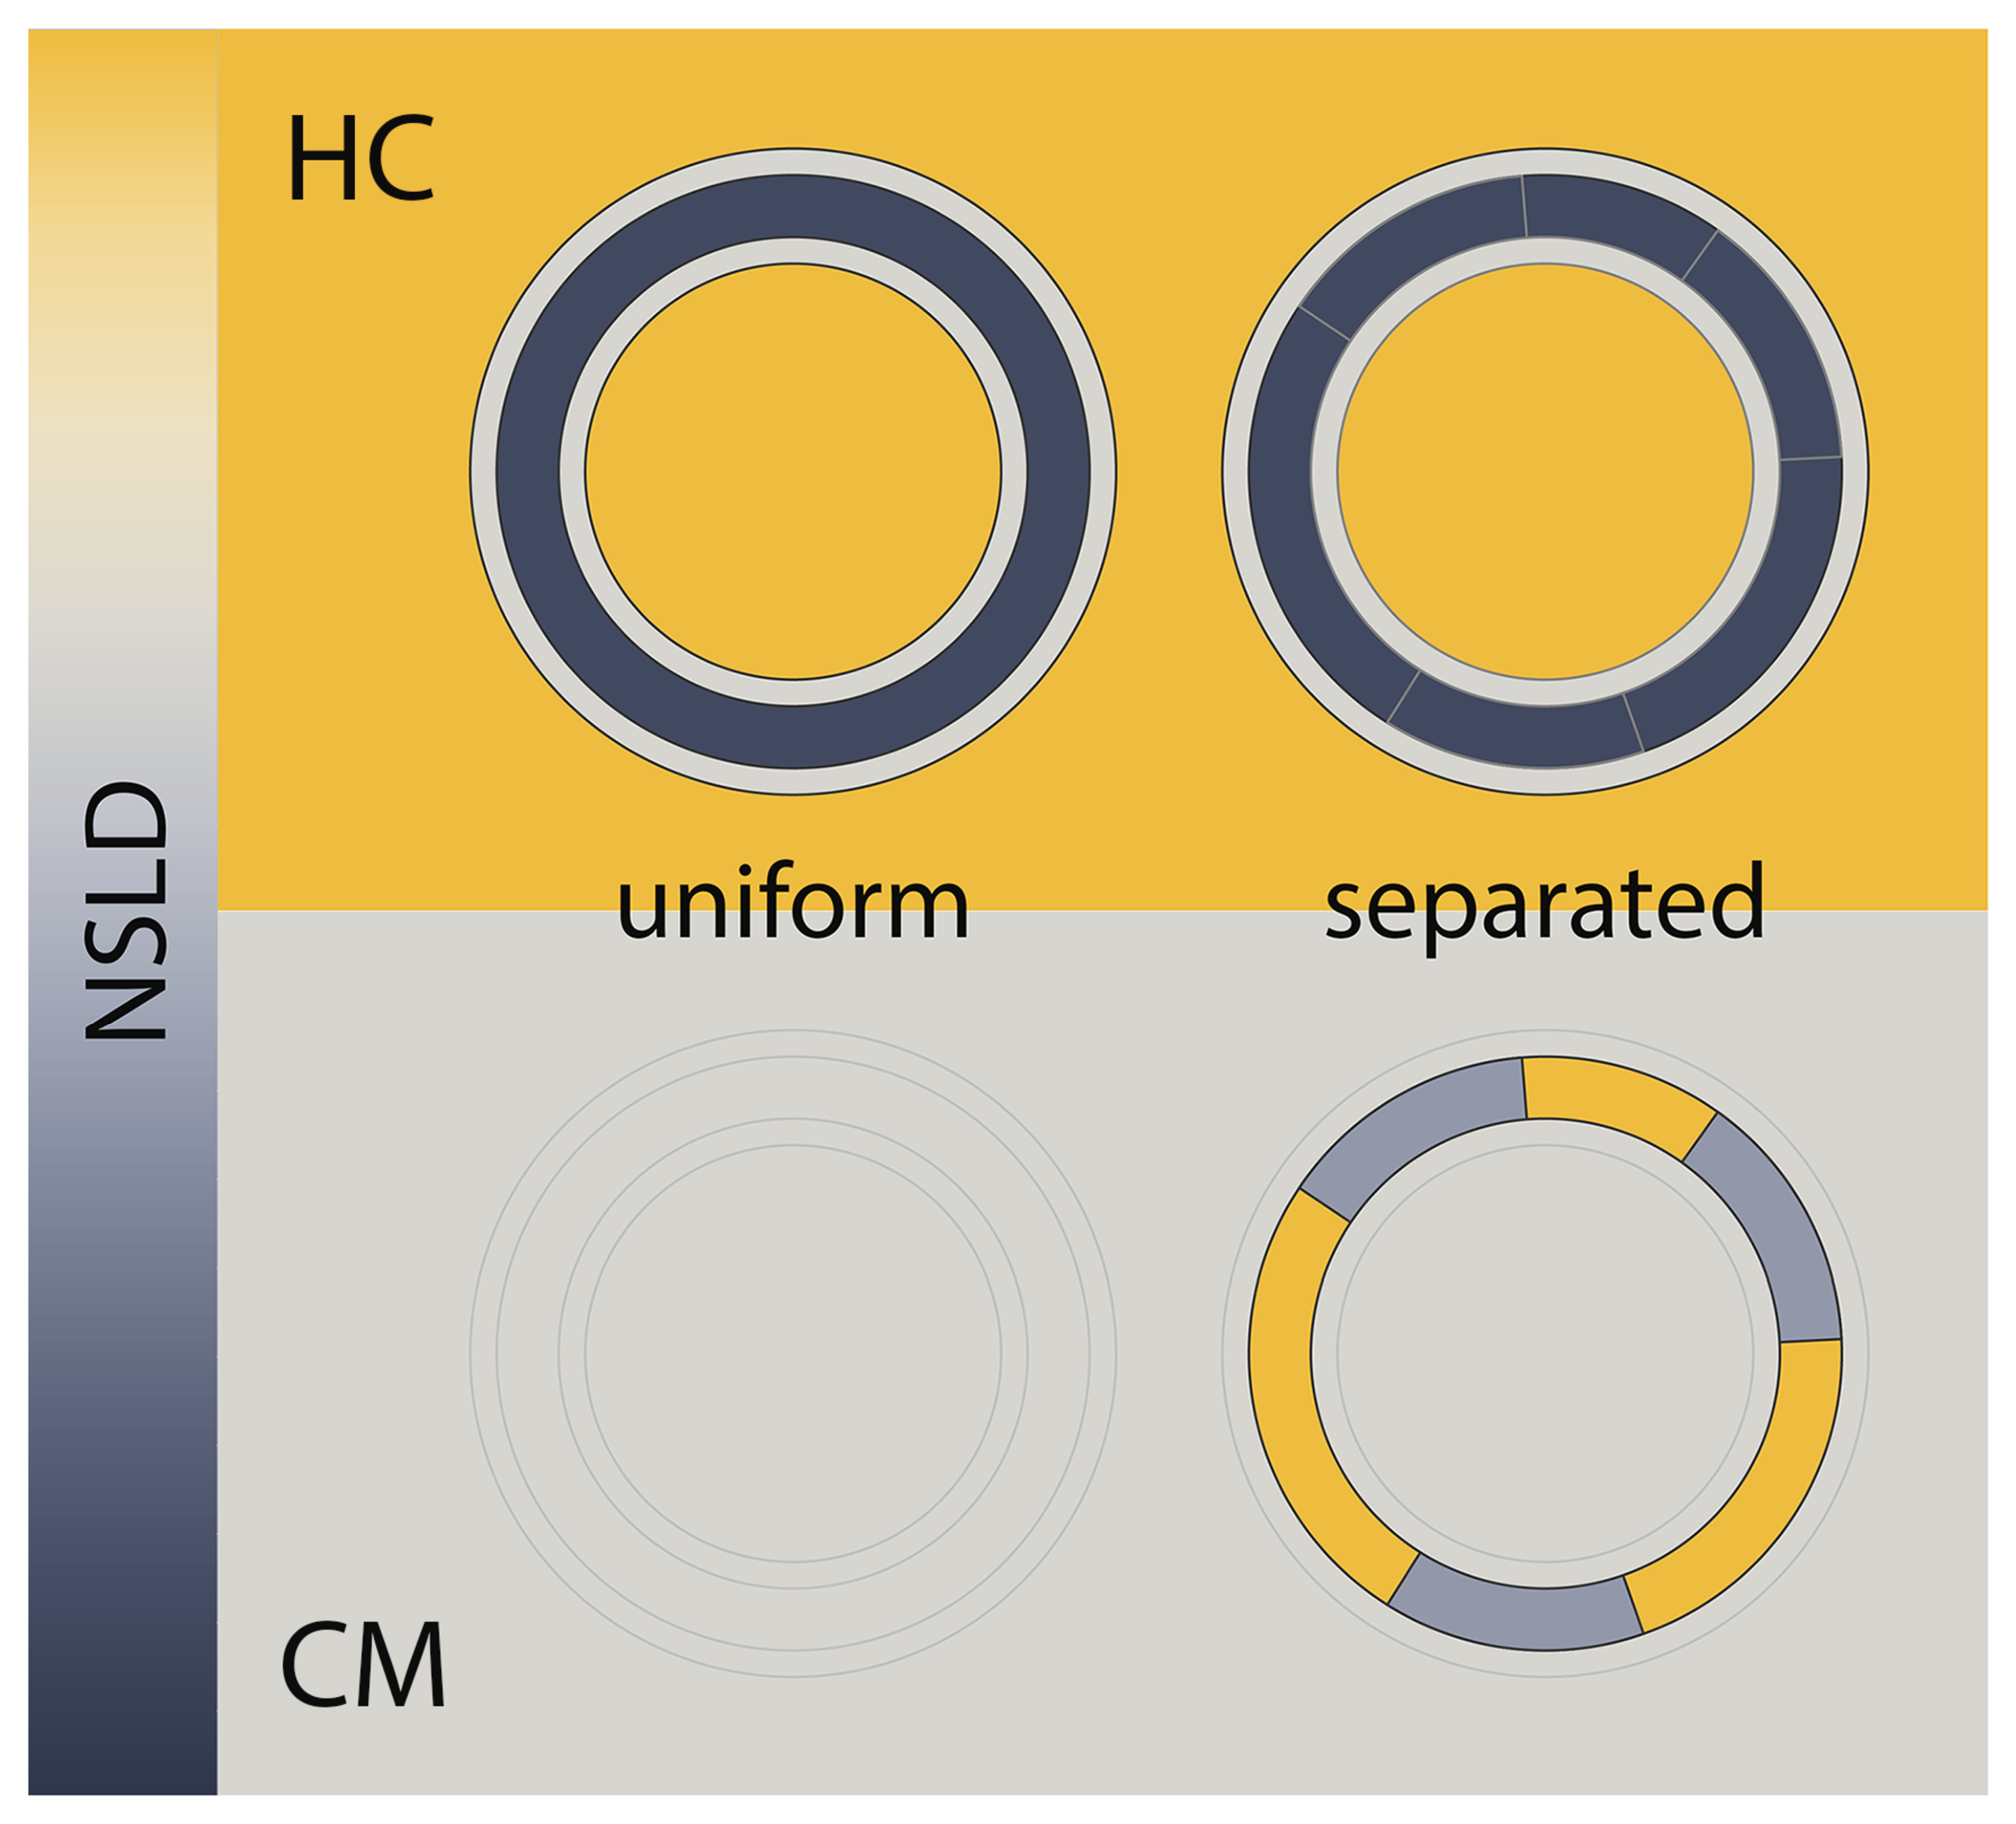
\includegraphics[width=0.4\textwidth]{figures/figure_1_contrast_schematic.eps}
	\caption{Detecting domains with neutron scattering requires optimizing contrast conditions. Neutron scattering length density (NSLD) is depicted as a continuous gradient between dark gray and yellow (left). The upper panel demonstrates a typical SANS experiment performed in 100\% D$_2$O solvent, using protiated lipids. In this ``high contrast'' (HC) scenario, a large NSLD difference exists between solvent and the lipid hydrocarbon region (with a smaller contrast between the lipid headgroup and hydrocarbon chains), and as such, lateral segregation of lipids (i.e., phase separation) results in no apparent change in contrast or scattered intensity (upper right). Through the use of chain perdeuterated lipids and solvent contrast variation, it is often possible to simultaneously match the SLD of the lipid headgroup, hydrocarbon chains, and water, as shown in the lower panel. In such a ``contrast matched'' (CM) sample, uniform lipid mixing results in a null scattering condition (lower left), but lateral segregation of chain protiated and chain perdeuterated species generates a lateral contrast (lower right), and hence an increase in scattering.}
	\label{fig:SANS_domains}
	
\end{figure}

Pencer et al. systematically addressed this problem by considering how the various SLD contrasts in a phase separated vesicle contribute to its total scattering signal~\cite{Pencer.2006}. Approximating the vesicle structure as a series of concentric shells corresponding to the inner headgroups, hydrocarbon, and outer headgroups, the following SLDs are calculated:


\begin{equation}
\label{eq.Fred1}
	\rho_h= \frac{\sum_{i} \chi_i b_{h,i}}{\sum_{i}\chi_i V_{h,i}}
\end{equation}

\begin{equation}
\label{eq.Fred2}
	\rho_{ac}= \frac{\sum_{i} \chi_i b_{ac,i}}{\sum_{i}\chi_i V_{ac,i}}
\end{equation}


\noindent where the subscripts $h$ and $ac$ refer, respectively, to the headgroup and acyl chain shells, $b$ is the coherent neutron scattering length, $V$ is the molecular volume, and $\chi_i$ is the bilayer mole fraction of lipid species $i$. Similarly, the average total bilayer SLD is given by:

\begin{equation}
\label{eq.Fred3}
	\bar{\rho}= \frac{\sum_{i} \chi_i (b_{h,i}+b_{ac,i})}{\sum_{i}\chi_i( V_{h,i}+V_{ac,i})}.
\end{equation}

For ULVs, the total scattering $\mathrm{Q=\int I(q) q^2 dq}$ (also called the Porod invariant) can be decomposed into three additive contributions related to: (1) the SLD contrast between the average vesicle composition and the solvent; (2) the radial SLD contrast between the lipid headgroups and acyl chains; and (3) the lateral SLD contrast arising from domains having a different average acyl chain composition. Defining these three respective contributions as $Q_0$, $Q_r$, and $Q_l$ (i.e., Q=$Q_0$+$Q_r$+$Q_l$), Pencer et al.~\cite{Pencer.2006} showed that:

\begin{equation}
\label{eq.Fred4}
	Q_0 \propto (\bar{\rho}-\rho_m)^2
\end{equation}

\begin{equation}
\label{eq.Fred5}
	Q_r \propto t_f(1-t_f)(\rho_{ac}-\rho_h)^2
\end{equation}

\begin{equation}
\label{eq.Fred6}
	Q_l \propto t_fa_f(1-a_f)(\rho_{Ld}-\rho_{Lo})^2
\end{equation}
where $\rho_m$ is the solvent SLD, $\rho_{Ld}$ and $\rho_{Lo}$ are the respective acyl chain SLDs of the L$_d$ and L$_o$ phases, $\mathrm{t_f=t_{ac}/(t_{ac}+2t_h)}$ is the ratio of the average acyl chain thickness to the total bilayer thickness, and $a_f$ is the vesicle surface area fraction occupied by domains. Importantly, the total homogeneous scattering contribution $Q_{hom}$=$Q_0$+$Q_r$ depends only on the solvent and averaged lipid SLDs, and not on the lateral distribution of lipids within the bilayer. In this sense, the homogeneous scattering is an undesirable background signal--for detecting domains, the optimal experimental condition corresponds to enhancing $Q_l$ and minimizing $Q_{hom}$ through contrast matching.

An instructive example of contrast matching is found in Heberle et al.~\cite{Heberle.2013}, where the authors examined domain formation in a series of lipid mixtures including DSPC/DOPC/Chol in a 39/39/22 ratio. At 20 $^\circ$C, this mixture separates into coexisting L$_d$ and L$_o$ phases, strongly enriched in DOPC and DSPC, respectively~\cite{Zhao.2007}. Though DOPC and DSPC have similar acyl chain NSLDs (Table ~\ref{tab:NSL}), a large contrast between L$_d$ and L$_o$ domains can nevertheless be generated by replacing DSPC with its chain perdeuterated counterpart, DSPC-d70. Introducing DSPC-d70 into the bilayer results in a large increase in $\rho_{Lo}$ but only a small increase in $\rho_{Ld}$, thereby enhancing the lateral scattering contribution $Q_l$ according to Eq.~\ref{eq.Fred6}. At the same time, the background homogeneous scattering $Q_{hom}$  is also affected, through changes in average acyl chain and bilayer SLDs ($\rho_{ac}$ and $\bar{\rho}$, respectively).

\begin{table} [b]
{\setlength{\tabcolsep}{4pt}
	\caption{Neutron scattering lengths, molecular volumes at 60 $^\circ$C, and scattering length densities of various lipid species.}
	\begin{tabular}{llccc}\hline
	 Molecule & Chemical & $b$ (fm) & $V$  & NSLD  \\
     &Formula & & (\AA$^3$) & (fm/\AA$^3$)\\
		\hline
		PC headgroup &	C$_{10}$H$_{18}$NO$_8$P & 60.1 & 331$^a$ & 0.181 \\
		DSPC chains & C$_{34}$H$_{70}$ & -35.8 & 1017$^b$ & -0.035 \\
		DSPCd70 chains & C$_{34}$D$_{70}$ & 692.9 & 1017$^b$ & 0.681 \\
		DOPC chains & C$_{34}$H$_{66}$ & -20.8 & 1003$^c$ & -0.021 \\
        POPC chains & C$_{32}$H$_{64}$ & -26.6 & 953$^b$ & -0.028 \\
        cholesterol & C$_{27}$H$_{46}$O & 13.3 & 630$^d$ & 0.021 \\
        water & H$_2$O & -1.68 & 30.4 & -0.055 \\
        heavy water & D$_2$O & 19.15 & 30.5 & 0.628 \\
        34.6\% heavy water& H$_{1.31}$D$_{0.69}$O & 5.53 & 30.4 & 0.181 \\
  
	\end{tabular}
    \label{tab:NSL}
    }
	\\
	{\footnotesize $^a$reference 4; $^b$reference 5; $^c$reference 6;  $^d$reference 7 }
\end{table}


\begin{figure} [t]
	\centering
	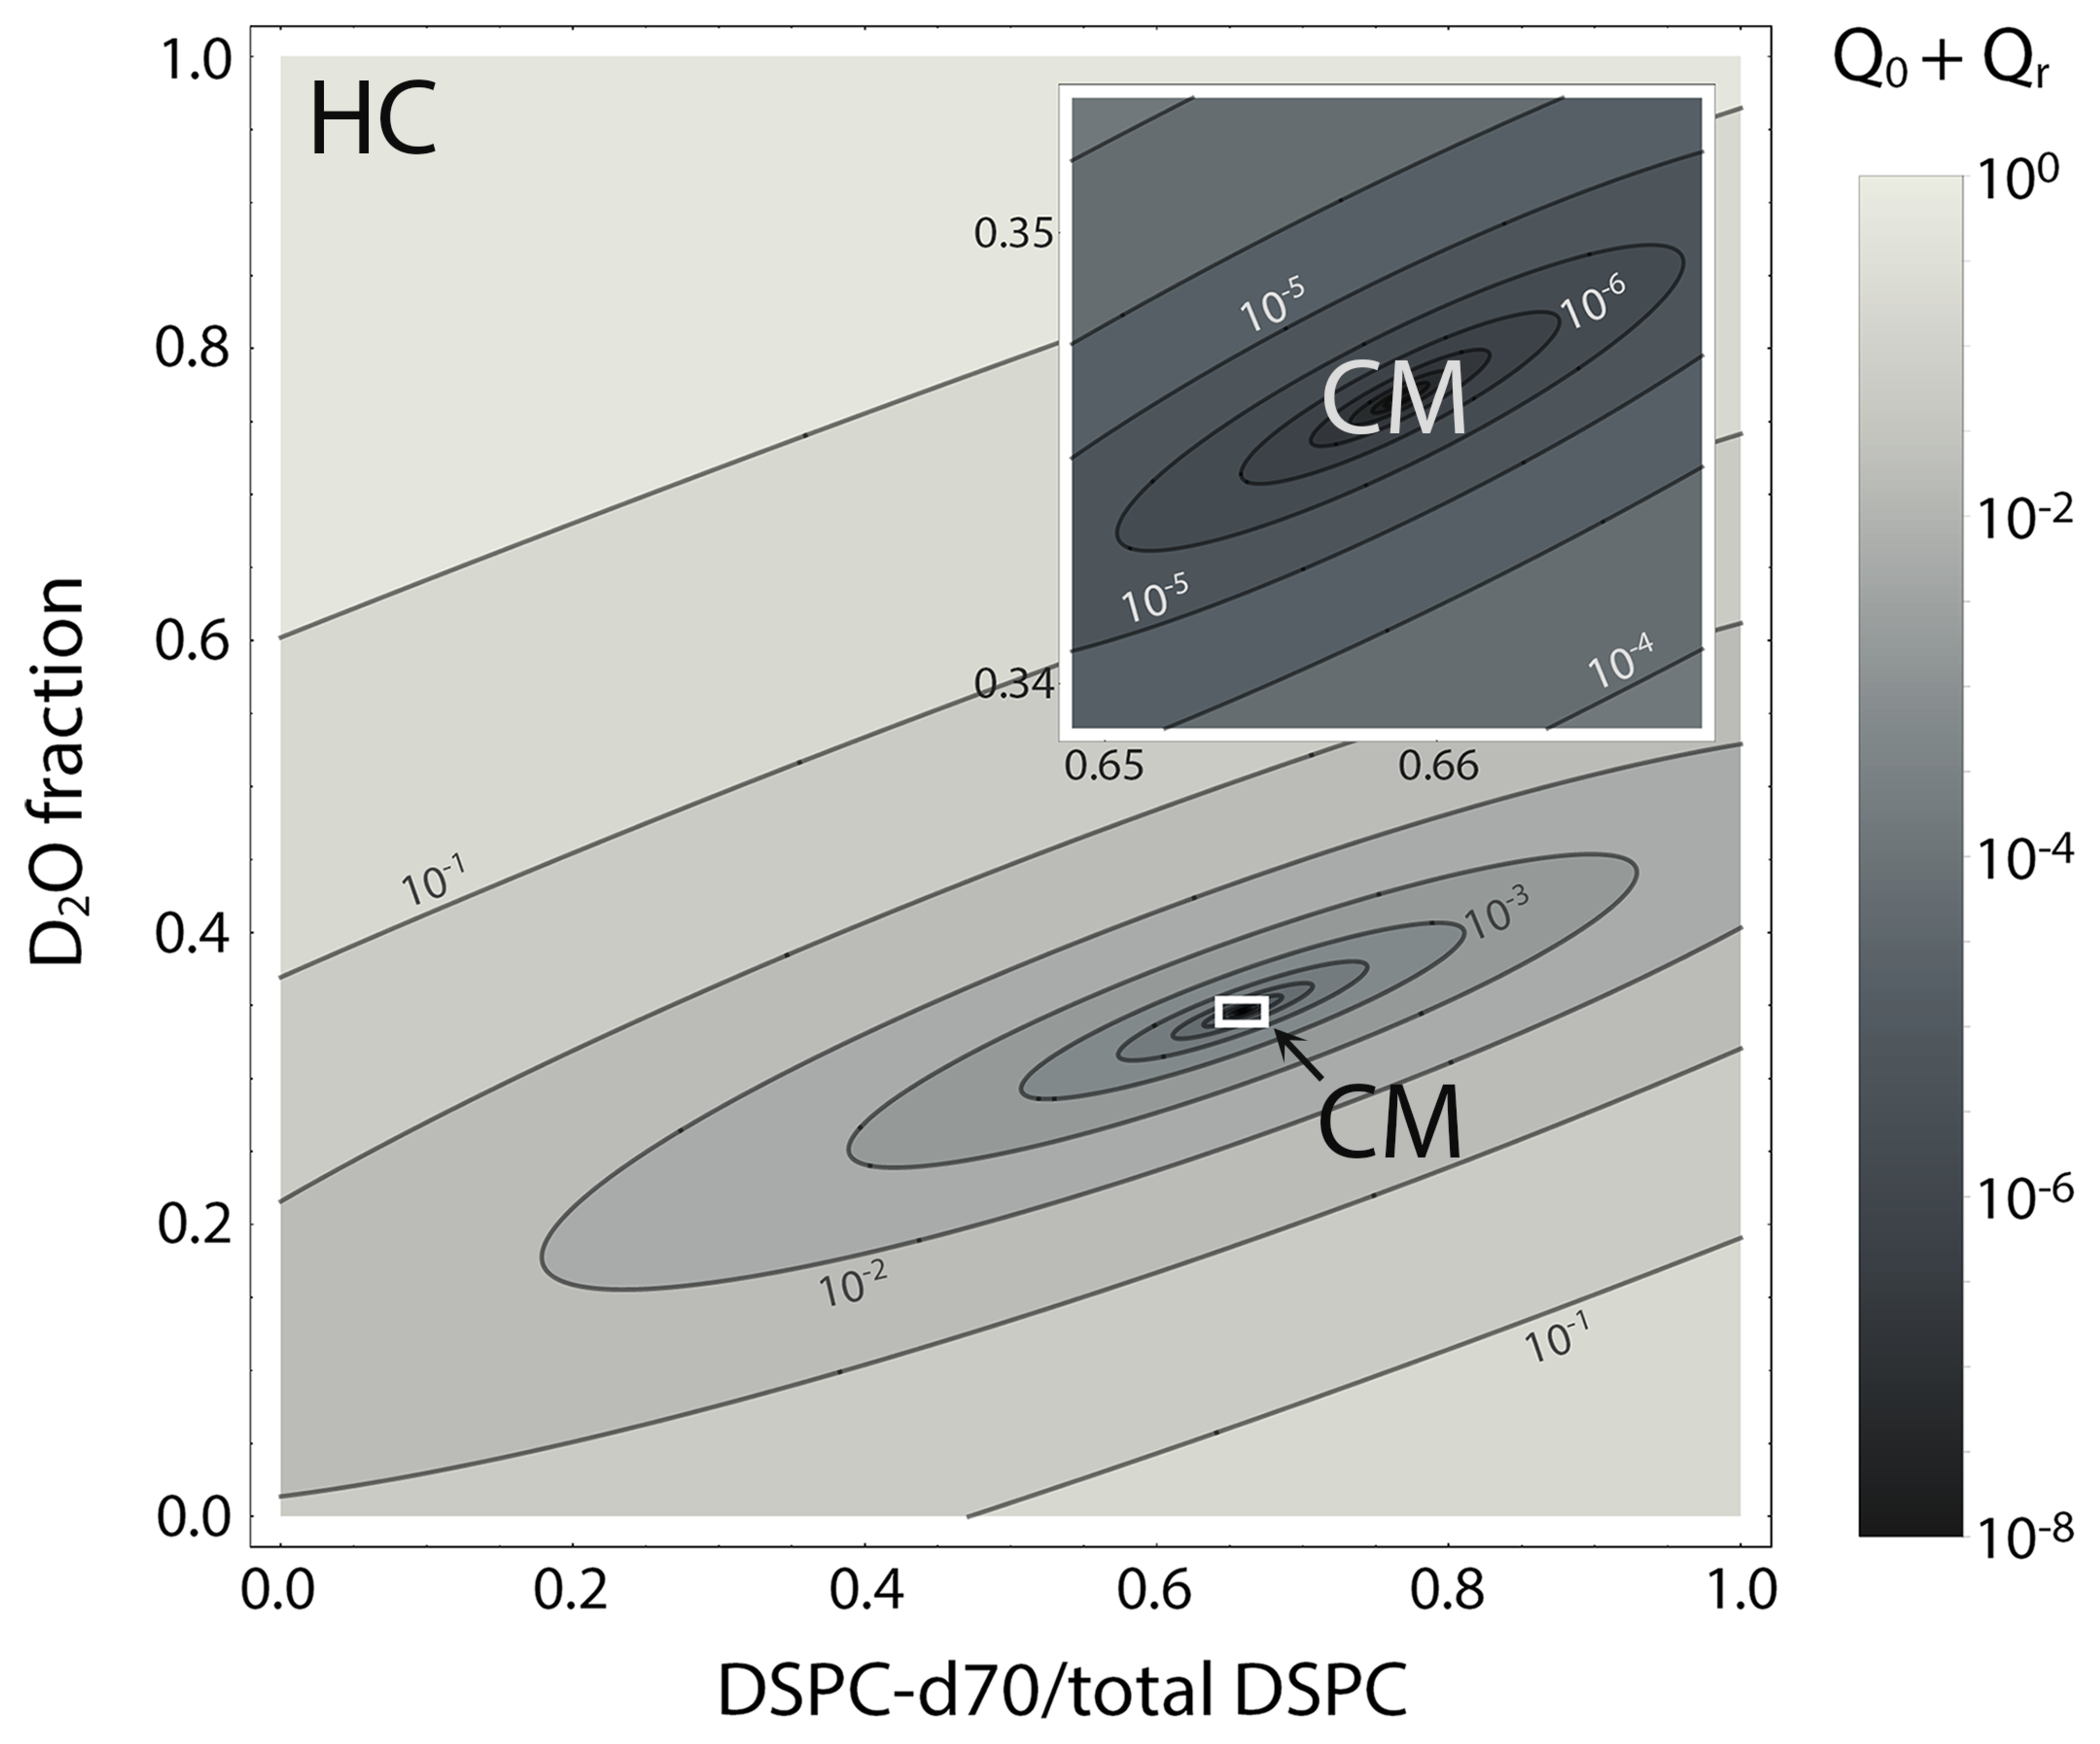
\includegraphics[width=0.4\textwidth]{figures/figure_2_contrast_match_contour.eps}
	\caption{Optimizing experimental conditions for detecting domains in DSPC/DOPC/Chol. The relative homogeneous background scattering $Q_{hom}$=$Q_0$+$Q_r$, calculated from lipid NSLDs (Table ~\ref{tab:NSL}) using Eqs.~\ref{eq.Fred1}-\ref{eq.Fred6}, is plotted \emph{vs}. fraction of DSPC-d70 (to total DSPC) and the solvent fraction of D$_2$O. A global contrast match point is observed at 34.6\% D$_2$O and 65.9\% DSPC-d70 (``CM'', expanded in inset). Close to the contrast match point, $Q_{hom}$ is attenuated by $>$ 6 orders of magnitude relative to a fully protiated bilayer in 100\% D$_2$O solvent (``HC'').}
	\label{fig:opt_exp_cond}
	
\end{figure}

 Figure ~\ref{fig:opt_exp_cond} shows a contour plot of $Q_{hom}$ \emph{vs} the fraction of DSPC-d70 (to total DSPC), and the solvent fraction of D$_2$O calculated using Eqs.~\ref{eq.Fred1}-\ref{eq.Fred6} and data from Table ~\ref{tab:NSL}. A sharp minimum in $Q_{hom}$ is observed at 34.6\% D$_2$O and 65.9\% DSPC-d70, precisely the point where the solvent and average bilayer NSLDs are matched to the PC headgroup. Using these experimental conditions, $\rho_m \cong \rho \cong \rho_h \cong \rho_{ac} \cong 0.181 fm/\AA^3$, and if the lipids are randomly mixed within the bilayer plane (e.g., at high temperature), a null scattering condition exists (Fig. \ref{fig:SANS_domains}, lower left). However, demixing of saturated and unsaturated lipids causes lateral NSLD fluctuations that generate in-plane contrast (Fig. \ref{fig:SANS_domains}, lower right), resulting in increased scattering according to Eq. \ref{eq.Fred6}.

Figure \ref{fig:porod} shows total scattering for several 4-component lipid mixtures studied at bilayer contrast matching conditions~\cite{Heberle.2013}. For mixtures containing DSPC and low-melting lipid (either POPC or DOPC) in a 1:1 ratio, in addition to 22 mol\% cholesterol, a marked increase in total scattering was observed with decreasing temperature, indicating domain formation. At fixed temperature, the magnitude of the Porod invariant showed a systematic decrease as POPC replaced DOPC, consistent with a reduction in domain area fraction, and weaker DSPC partitioning between the L$_d$ and L$_o$ phases~\cite{Heberle.2010,Konyakhina.2013}. In contrast, single phase mixtures showed low total scattering and little variation over the temperature range studied.

\begin{figure} [t]
	\centering
	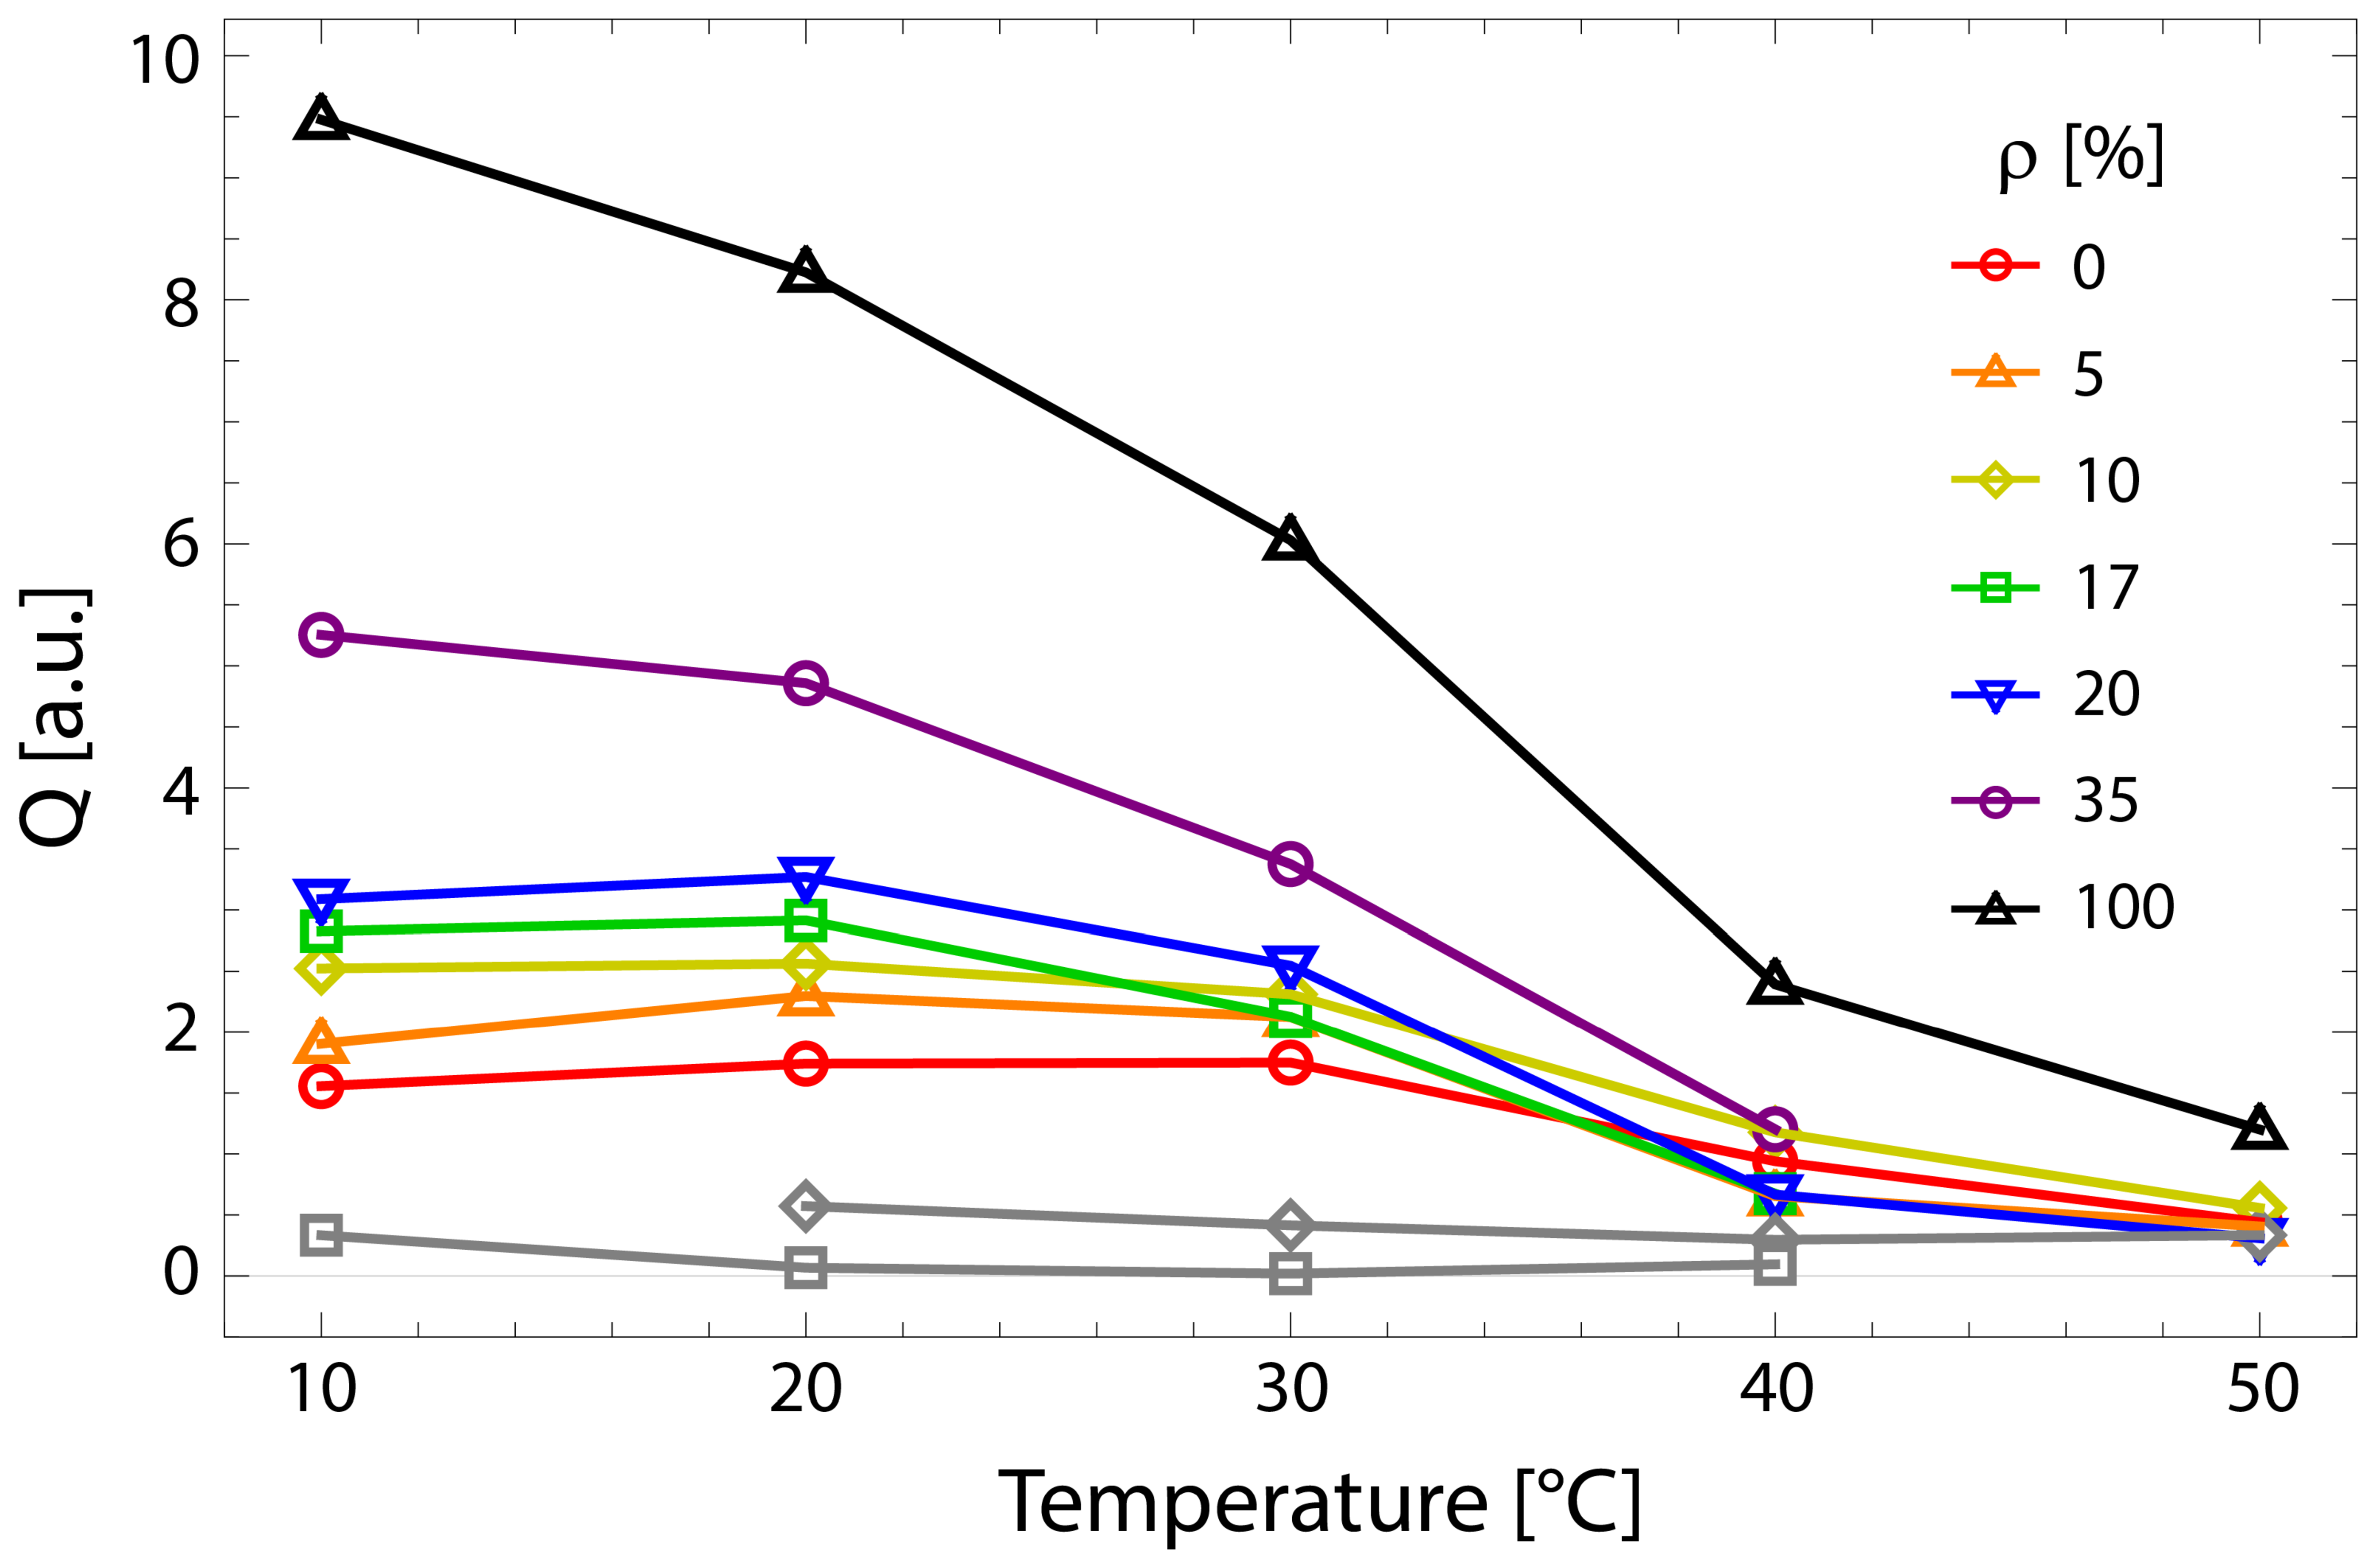
\includegraphics[width=0.4\textwidth]{figures/figure_3_porod.eps}
	\caption{Total scattering reveals domain formation in 4-component lipid mixtures. Shown is the Porod invariant Q plotted vs. temperature for DSPC/(DOPC+POPC)/Chol mixtures in a 0.39/0.39/0.22 molar ratio. Colors correspond to different values of the composition parameter $\mathrm{\rho=\chi_{DOPC}/(\chi_{DOPC}+\chi_{DOPC})}$ as indicated in the legend. Also shown are two single-phase control samples: DSPC/POPC/Chol 0.325/0.325/0.35 (gray diamond) and POPC/Chol 0.65/0.35 (gray square).}
	\label{fig:porod}
	
\end{figure}

As a model-free method, the Porod invariant is a robust diagnostic tool for probing lateral bilayer inhomogeneities~\cite{Heberle.2013,RobinS.Petruzielo.2013}. However, this strength is at the same time a weakness--by collapsing the $q$-dependence of the scattering signal, any potential information regarding the size, shape, and spatial distribution of domains is lost. Elucidating these details requires modeling $I(q)$, as will be discussed in the next section.

\subsubsection{Analytical form factor. }
An analytical solution for domain scattering was first provided by Anghel et al.~\cite{Anghel.2007}, in which the authors used a spherical harmonic expansion of the scattering amplitude to derive the form factor of a vesicle containing a single round domain. However, this model proved inadequate for describing experimental SANS data in the well-studied domain forming mixtures DPPC/DOPC/Chol~\cite{Pencer.2005} and DSPC/(DOPC+POPC)/Chol~\cite{Heberle.2013}. In both studies, Monte Carlo analyses instead suggested the presence of multiple domains in ULVs. To facilitate the study of such systems, the analytical form factor was recently generalized to static configurations of multiple, arbitrarily sized domains, with the ability to accommodate distributions of domain sizes or configurations through appropriate averaging (Heberle et al. 2015 J. Appl. Cryst. (submitted)). To illustrate the general model, we now consider the solution for uniformly sized round domains.

	The scattered intensity of a vesicle containing multiple domains can be expressed as:

\begin{equation}
\label{eq.Fred7}
	I(q) = I_{hom}(q) +I_{intra}(q) + I_{inter}(q)
\end{equation}
The first term in Eq.~\ref{eq.Fred7} comprises the homogeneous contribution to the total scattering, arising from radial SLD contrasts of each phase:


\begin{equation}
\label{eq.Fred8}
	I_{hom}(q) = \left[M_0(q) + \frac{N_d(1-\cos\alpha_d)}{2}W_0(q)\right]^2
\end{equation}

\begin{equation}
\label{eq.Fred9}
	M_0(q) = \int^{\infty}_0 [\rho_c(r)-\rho_m]r^2j_0(qr)dr
\end{equation}


\begin{equation}
\label{eq.Fred10}
	W_0(q) = \int^{\infty}_0 [\rho_d(r)-\rho_c(r)]r^2j_0(qr)dr
\end{equation}
Here, subscripts $d$ and $c$ refer, respectively, to the domain and continuous phases, $N_d$ is the number of domains, $\alpha_d$ is the angle formed by vectors pointing from the vesicle center to the domain center and edge, and $j_0$ is the zeroth order Bessel function. Equation \ref{eq.Fred9} is recognized as the core/shell (i.e., vesicle) form factor for the continuous phase, and is calculated as the Fourier transform of its radial SLD profile, while Eq.~\ref{eq.Fred10} represents the Fourier transform of the radial SLD \emph{difference} between the domain and continuous phases. The second term in Eq.~\ref{eq.Fred7} describes intra-domain scattering arising from domain self-correlation:

\begin{equation}
\label{eq.Fred11}
	I_{intra}(q) = N_d \sum_{l=1}^{\infty}|\tilde{w}_l^0(\alpha_d)|^2|W_l(q)|^2
\end{equation}

\begin{equation}
\label{eq.Fred12}
	W_l(q) = \int^{\infty}_0 [\rho_d(r)-\rho_c(r)]r^2j_l(qr)dr
\end{equation}


\begin{equation}
\label{eq.Fred13}
	\tilde{w}_l^0(\alpha_d) = \frac{\sqrt{(2l+1)}}{2l}[\cos\alpha_dP_l(\cos(\alpha_d)- P_{l+1}(\cos\alpha_d)]
\end{equation}
where $P_l$ is the Legendre polynomial of degree $l$. Finally, the third term in Eq.~\ref{eq.Fred7} accounts for inter-domain scattering, arising from coherent interference between different domains:

\begin{equation}
\label{eq.Fred14}
	I_{inter}(q) = \sum_{J\neq K} \sum_{l=1}^{\infty}|\tilde{w}_l^0(\alpha_d)|^2|W_l(q)|^2P_l(\cos\theta_{JK})
\end{equation}
where $\theta_{JK}$ is the angle between the vesicle center and the centers of domains $J$ and $K$. Equation \ref{eq.Fred14} reveals that the inter-domain scattering contribution depends solely on the relative spatial configuration of domain pairs.


\begin{figure} [t]
	\centering
	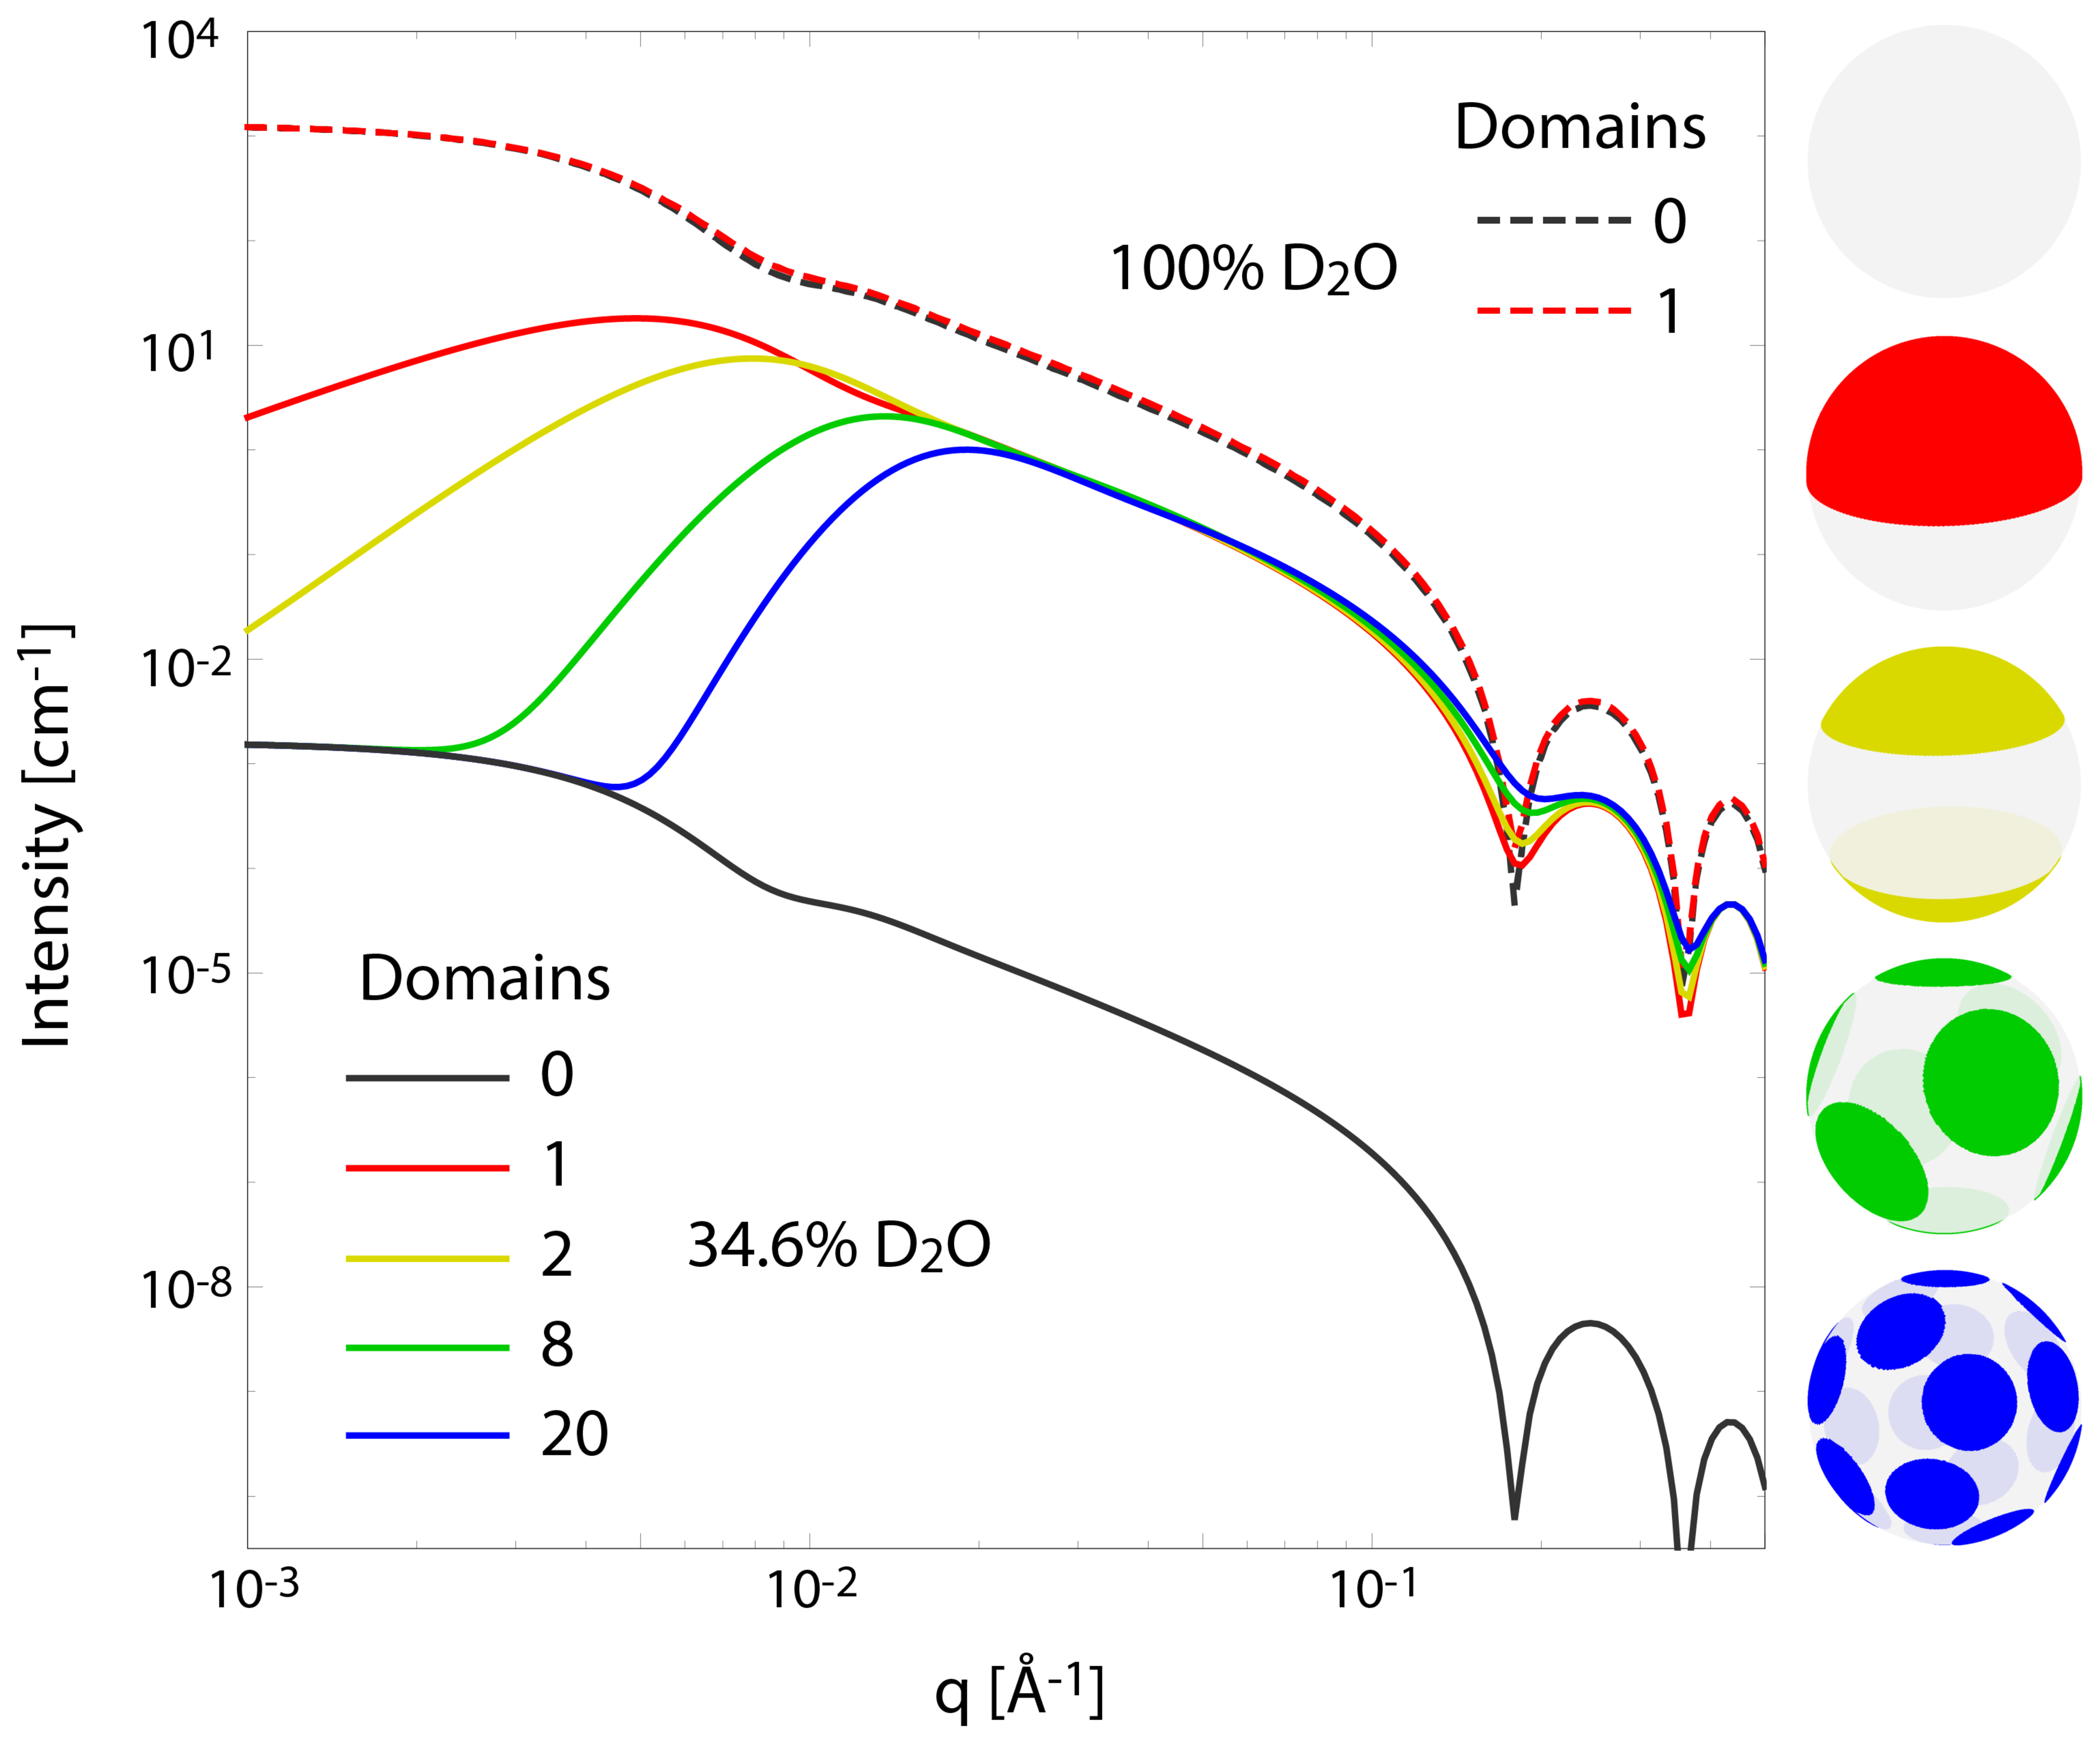
\includegraphics[width=0.4\textwidth]{figures/figure_4_analytical_model.eps}
	\caption{Analytically calculated scattered intensity for multiple round domains. For all curves shown, the total bilayer NSLD is identical--differences in scattered intensity are due to differences in solvent NSLD and/or the lateral NSLD distribution, as indicated by the figure legend and color-coded vesicle images (right). At 100\% D$_2$O, the homogeneous scattering dominates and little difference is apparent between a uniform (black dashed) and phase-separated (red dashed) vesicle. At 34.6\% D$_2$O, the mean and radial scattering contributions are minimized, resulting in a reduction in the homogeneous scattering component by 6 orders of magnitude (black solid line). Phase separation now results in a dramatic increase in coherent scattered intensity, which depends on the size and configuration of domains (colored solid lines).}
	\label{fig:analytical}
	
\end{figure}

Figure \ref{fig:analytical} illustrates the analytical model given typical experimental conditions, in this case corresponding to the DSPC/DOPC/Chol mixture described above. For all curves, the total bilayer NSLD is identical, and differences in scattered intensity are due either to differences in solvent SLD, or the presence (or absence) of domains. At 100\% D$_2$O, there is little apparent difference between uniform (black dashed) and phase-separated (red dashed) vesicles. However, consistent with the prediction of Fig. \ref{fig:opt_exp_cond}, the differences are greatly magnified near the contrast match point (solid curves). While scattering from a uniformly mixed vesicle exhibits the same relative $q$-dependence at 100\% and 34.6\% D$_2$O (black dashed and solid curves, respectively), the total homogeneous intensity is attenuated by a factor of nearly 10$^6$ near the contrast match point. Now, phase separation results in a 10$^4$-fold increase in scattered intensity (colored solid curves), with a distinct peak evident in the low-$q$ regime ($q$ $<$ 0.1 \AA$^{-1}$). Upon increasing the number of domains, at a fixed total domain area fraction of 0.5 (i.e., decreasing the domain size), this peak steadily shifts to higher $q$ (yellow, blue, and green curves), an effect that was previously observed experimentally~\cite{Heberle.2013,Heberle.2013b}. In the high-$q$ regime ($q$ $>$ 0.1 \AA$^{-1}$), substantially increased intensity or ``liftoff'' is observed near the minima between scattering lobes, which increases with increasing number of domains. Such liftoff is typically interpreted as evidence for transbilayer asymmetry~\cite{Kucerka.2007,Brzustowicz.2005}, but clearly can also originate from lateral SLD fluctuations, especially in SANS experiments utilizing mixtures of protiated and deuterated lipids.

\subsection{Inelastic neutron scattering}
Inelastic neutron scattering offers an experimental approach for the determination of bilayer mechanical properties (see sec. \ref{InES}). Recent studies have used bilayer dynamics to probe the bending modulus of different homogenously mixed lipid bilayers~\cite{Woodka.2012,Pan.2015,Yi.2009}. This technique has also been used to show how the bending modulus is affected by a number of parameters including charge density~\cite{Bruning.2013}, cholesterol content~\cite{Arriaga.2010}, and the presence of pore forming peptides~\cite{Lee.2010}, to name a few. In order to investigate the mechanical properties of phase separated lipid bilayers \textit{in situ}, a forthcoming work~\cite{Nickels.2015b} has employed inelastic neutron scattering to study the mechanical properties of nanoscopic domains. Building on the demonstrated ability to induce neutron contrast in phase separated ULVs~\cite{Heberle.2013}, the SLD of an individual phase (L$_o$) was matched to that of the solvent. In this way, it is possible to isolate the scattering of the non-contrast matched phase (L$_d$), enabling the study of nanoscopic lipid domains. This scheme enabled a series of SANS, diffraction, and inelastic scattering experiments that revealed nanoscopic domains to be in registry, and that the bending modulus of nanoscopic lipid domains \textit{in situ} closely matches that of the pure L$_d$ phase. From these measurements, Nickels et al.~\cite{Nickels.2015b} were also able to observe important interfacial phenomena at the domain boundary, and the profound role that  bending energy has on the thermodynamics of phase separation. 


\subsection{Elastic X-ray scattering}
\label{sec:elatic_xray}
\subsubsection{SAXS. }
In the case of x-rays, there is no appreciable lateral contrast enabling them to detect domains. However, x-rays are highly sensitive to electron density variations across the bilayer, and consequently to the internal structure of domains. In order to probe domain structure \textit{in situ}, it is best done using multibilayer stacks. In this sample preparation, like-domains are in registry and can be detected as two separated lamellar lattices if $V_{coh} < D$ (Fig.~\ref{fig:SAXS_domains}). This is typically the case for macroscopic domains on the order of a few $\mu$m.

\begin{figure} [t]
	\centering
	\includegraphics[height=9cm]{figures/SAXS_domains.pdf}
	\caption{L$_o$/L$_d$ phase coexistence as detected by SAXS. Like domains exhibit long-range alignment and consequently display two distinct lamellar lattices. Here $\circ$'s indicate peaks associated with L$_o$ domains and $\times$'s peaks associated with L$_d$ domains.  The inset to the scattering pattern of DSPC/DOPC/Chol in the phase coexistence regime shows the EDP of the two domains resulting from a global fit (red solid line). Figure taken from~\cite{Heftberger.2015b}.}
	\label{fig:SAXS_domains}
	
\end{figure}

For MLVs Heftberger et al.~\cite{Heftberger.2015} demonstrated that the scattered intensity of such systems can be modeled as:
\begin{equation}
	I(q)= \left(1-c_{Ld}\right) I_{Lo}(q)+ c_{Ld} I_{Ld}(q),
\end{equation}
where $c_{Ld}$ accounts for the L$_{d}$ phase fraction, and $I_{Lo}$ and $I_{Ld}$ are the scattered intensities of the liquid ordered and liquid disordered phases, respectively, and are given by Eq.~(\ref{eq:SDP_GAP}). Thus, every phase is described by a separate structure factor (Eq.~\ref{eq:caille}) and form factor (Eq.~\ref{eq:SDP_formfac}). Due to the presence of a high-T$_m$ lipid and the condensing effect of cholesterol L$_o$ phases are considerably more rigid than L$_d$ domains. Thus, their Caill\'{e} parameter is about 65\% smaller (Tab.~\ref{tab:results_Ld-Lo}) and the number of Bragg peaks is almost double that of those associated with the L$_d$ phase (Fig.~\ref{fig:SAXS_domains}).

Having established the SDP analysis for MLVs~\cite{Heftberger.2014} (see also above), it is more or less straight forward to extend this model to coexisting domains. However, since each domain has a characteristic lipid composition (in the case of ternary mixtures, a high-$T_m$ lipid, a low-$T_m$ lipid and cholesterol) the underlying parsing scheme of quasi-molecular fragments needs to average over the contributions of each lipid, as illustrated in Fig.~\ref{fig:SAXS_parsing_domains}. 

\begin{figure} [t]
	\centering
	\includegraphics[height=9cm]{figures/parsing_scheme_domains.pdf}
	\caption{Parsing scheme of ternary lipid mixtures based on MD simulations of an $L_o$ phase (panel A, DPPC lipids are drawn in blue, DOPC in red, and cholesterol in yellow). Panel B shows the electron density profile calculated from simulations, and panel C the electron densities of individual molecular groups. The left side panel shows the individual contributions of DPPC (solid lines) and DOPC (dashed lines) for the CholCH$_3$, PCN, CG, CH$_2$ and CH$_3$ groups. The contribution of cholesterol is shown as a separate yellow line. The panel on the right shows the condensed parsing scheme after merging individual contributions. Figure taken from~\cite{Heftberger.2015} with permission.}
	\label{fig:SAXS_parsing_domains}
\end{figure}


\begin{table} [b]
	\caption{Structural results and bending fluctuations for coexisting $L_d/L_o$ domains~\cite{Heftberger.2015}. Parameter uncertainties are $<$2\,\%}
	\begin{tabular}{lccc}\hline
		 & $d_B$ (\AA) & $A$ (\AA$^2$) & $\eta$ \\
		\hline
		DOPC/DPPC/Chol$^a$-L$_d$ &	37.9 & 64.9	& 0.074 \\
		DOPC/DPPC/Chol$^a$-L$_o$ &	47.2 & 44.4	& 0.021 \\
		DOPC/DSPC/Chol$^b$-L$_d$ &	38.5 & 63.1	& 0.091 \\
		DOPC/DSPC/Chol$^b$-L$_o$ &	49.8 & 43.2	& 0.030 \\
	\end{tabular}
	\label{tab:results_Ld-Lo}
	\\ \\
	{\footnotesize $^a$Molar fractions: DOPC (0.37), DPPC (0.47), Chol (0.16), T = 15$^\circ$C \\
		$^b$Molar fractions: DOPC (0.42), DSPC (0.37), Chol (0.21), T = 22$^\circ$C}
\end{table}

In order to establish this analysis, results from tieline endpoint samples were compared with tieline midpoint samples and yielded -- within experimental uncertainty -- good agreement~\cite{Heftberger.2015}. Results of the \textit{in-situ} study of DOPC/DPPC/Chol and DOPC/DSPC/Chol showed that L$_o$ domains are about 9-10 \AA\/ thicker than L$_d$ phases, and that their area per lipid is about 20 \AA$^2$ smaller (Tab.~\ref{tab:results_Ld-Lo}). Further increase to the overall cholesterol concentration decreased the differences between L$_o$ and L$_d$. This suggests that the L$_o$ phase is saturated with cholesterol, and that additional cholesterol incorporates itself into the L$_d$ phase.

Heftberger and co-workers~\cite{Heftberger.2015} additionally studied the temperature behavior of phase separated systems across the transition to a homogeneous phase (Fig.~\ref{phase_diagram}). In SAXS, this event is observed as a merging of the lamellar diffraction peaks (Fig.~\ref{fig:Lo_melting}). Analysis of the corresponding diffraction patterns showed that melting of the L$_o$ phase is associated with a decrease in bilayer thickness, and an increase in area per lipid and bending fluctuations. This is typical of fluid phase bilayers~\cite{Pabst.2004,Kucerka.2011}. In contrast, L$_d$  show an exact opposite behavior (i.e., increased $d_B$, and a decrease in $A$ and $\eta$)~\cite{Heftberger.2015}. The most likely explanation for these reported findings is that cholesterol diffuses at temperatures below $T_c$, from the L$_o$ to the L$_d$ phase. This process is accelerated as $T_c$ is approached from below, in agreement with a previous NMR observation~\cite{Davis.2014}.


\begin{figure} [t]
	\centering
	\includegraphics[height=7cm]{figures/Lo_melting.pdf}
	\caption{Melting of L$_o$ domains in DOPC/DSPC/Chol. Panel A shows a contour plot of second order Bragg reflections associated with $L_o$ and $L_d$ phases. Above $T_c$, only a single lamellar lattice is observed. Panel B shows Bragg scattering from L$_o$ (dashes) and L$_d$ (crosses) domains at 22$^\circ$C. Panel C is the same system at 50$^\circ$C. Best fits are shown as solid lines. Inserts to both panels show the resulting ED profiles for $L_o$ and $L_d$ phases. Figure taken from~\cite{Heftberger.2015} with permission.}
	\label{fig:Lo_melting}
\end{figure}

The in-situ analysis of coexisting phases detailed above relies on long-range positional correlations of like-domains in multibilayers. Such order has been directly observed using depth-resolved confocal microscopy~\cite{Tayebi.2012}. This poses a challenging scientific question: ``\textit{Why are the observed domains in registry?}''

The answer to this question is intimately coupled to the forces present between the domains. In the case of neutral membranes, the fundamental interactions are van der Waals, hydration, and undulation repulsion~\cite{Israelachvili.2011}. The fact that SAXS is able to differentiate between coexisting L$_o$ and L$_d$ domains offers the possibility to distinguish between these interaction using osmotic stress experiments. In such experiments, osmotic pressure is induced by large neutral polymers, such as polyethylene glycol~\cite{Parsegian.1986}. Due to their size, the polymers are excluded from the interbilayer water layer creating osmotic pressure that decreases bilayer separation. Bilayer separation as a function of osmotic pressure is then measured using SAXS (see e.g.~\cite{McIntosh.1993,Parsegian.1995}), and the data is fitted using functional forms of interaction potentials, which then yield the underlying inter-membrane forces. However, when entropically driven bending undulations are present, the standard Derjaguin-Landau-Verwey-Overbeek (DLVO) paradigm, which allows for the treatment of solvent-mediated interactions, is not applicable ~\cite{Israelachvili.2011}.

This, however, can be addressed by mean-field/additivity approximations, where conformational fluctuation effects on the
bare interaction potentials are included in a self-consistent manner~\cite{Sornette.1986,Evans.1986,Podgornik.1992,Mecke.2003}. Moreover, through measurements of the Caill\'{e} parameter the mean square fluctuations of the bilayer separation
%
\begin{equation}
	\Delta^2 = \frac{\eta d^2}{\pi^2}
\end{equation}
%
can be derived as a function of osmotic pressure by SAXS, allowing one to separate fluctuation contributions from bare interactions~\cite{Petrache.1998}.

A different approach from the above is Monte Carlo (MC) simulations~\cite{Gouliaev.1998,Gouliaev.1998b}. Recently, Kollmitzer et al.~\cite{Kollmitzer.2015} explored this approach for coexisting L$_o$/L$_d$ domains, by coupling MC simulations (Fig.~\ref{fig:MC_simulations}) to an optimization routine that jointly fits osmotic pressure dependencies of $d_W$ and $\Delta$. This allowed for the disentanglement of the different force contributions. Results (Fig.~\ref{fig:MC_simulations}) for this analysis show only small differences in the van der Waals interactions between L$_o$ and L$_d$. However, the other two interactions differed significantly. L$_o$ phases show a rapid decay of undulation repulsion (i.e., reduced fluctuations compared to L$_d$ phases), but a much slower decay in hydration repulsion. It is therefore clear that in the case of L$_d$ domains fluctuation forces dominate domain interactions over a broad range of distances, while hydration forces are most prominent in the L$_o$ phase. Thus, there seems to be a delicate balance between hydration and fluctuation interactions which underlies domain alignment, and this needs to be considered in future theoretical considerations on this subject.

\begin{figure} [t]
	\centering
	\includegraphics[height=3.5cm]{figures/MC_simulations.pdf}
	\caption{Real-space snapshots of equilibrium L$_d$ simulations at a given osmotic pressure. Figure taken from~\cite{Kollmitzer.2015} with permission.}
	\label{fig:MC_simulations}
\end{figure}

\begin{figure}
	\centering
	\includegraphics[height=7cm]{figures/forces.pdf}
	\caption{Deconstruction of the total osmotic pressure, $P$, into contributions of hydration, $P_{hyd}$, van der Waals, $P_{vdw}$, and undulation interactions, $P_{und}$, for coexisting L$_d$ (upper) and L$_o$ (lower) domains. Open black circles show the $d_W$ values at which the hydration and undulation pressures are equal. Figure taken from~\cite{Kollmitzer.2015} with permission.}
	\label{fig:forces}
\end{figure}

A further benefit from the above analysis is that the domain bilayer bending rigidity, $K_c$, can be derived from the fluctuation contributions. This is an important parameter with regard to the partitioning of proteins in either L$_o$ or L$_d$ domains~\cite{Marsh.2007,Marsh.2008}. For DOPC/DSPC/Chol, Kollmitzer and co-workers~\cite{Kollmitzer.2015} reported $K_c = 120$ zJ for L$_o$ and $44$ zJ for L$_d$ domains. In other words, L$_d$ domains are about three times softer than their L$_o$ counterparts.


\subsubsection{WAXS. }

Wide-angle x-ray scattering (WAXS) reports on chain-chain positional correlations -- peak position reflects the average distance between chains, while peak width is inversely related to in-plane positional correlations. The condensing effect of cholesterol shifts and broadens the WAXS peaks of PC bilayers, but even at high cholesterol concentration ($> 30$ mol\%) they resemble fluid bilayers~\cite{Engelman.1972}. Importantly, however, is that phase coexistence may be present even if only a single lamellar phase is seen in SAXS (e.g., this is because the $d$ spacings of both phases are the same, or $V_{cho}^{x-ray} \ge D$, see above). WAXS from oriented samples offers distinct advantages for examining phase separation. In such systems, off-axis scattering intensity is related to the distribution of acyl chain tilt angles, and the width of this distribution gives rise to an x-ray order parameter~\cite{Mills.2008b,Mills.2008}
%
\begin{equation}
	S_{x-ray}=\frac{1}{2} \left(3 <\cos^2 \beta >-1\right),
\end{equation}
%
where $\beta$ is the average tilt angle. $S_{x-ray}$ is markedly different for L$_d$ and L$_o$ phases. It should be pointed out that the absolute magnitude of $S_{x-ray}$ is different from the NMR carbon-deuterium order parameter $S_{CD}$ obtained from NMR~\cite{Mills.2008b}. Mills and coworkers~\cite{Mills.2008} applied this analysis to DOPC/DPPC/Chol mixtures (Fig.~\ref{fig:WAXS_domains}). In the phase coexistence regime they found that two tilt distributions were required to model the data (Fig.~\ref{fig:WAXS_domains}B) resulting in $S_{x-ray} \sim 0.7$ for L$_o$ and $S_{x-ray} \sim 0.4$ for L$_d$ domains, while only single order parameter was needed at temperatures $T > T_c$ and for binary DOPC/DPPC mixtures (Fig.~\ref{fig:WAXS_domains}A and C). 

\begin{figure}
	\centering
	\includegraphics[height=5cm]{figures/WAXS_domains.pdf}
	\caption{WAXS scattering from: (A) 1:1 DOPC/DPPC; and (B and C) 1:1 DOPC/DPPC/Chol (15 mol\%), T = 25$^\circ$C and 45$^\circ$C ($T_c \simeq 30$$^\circ$C). The bottom row shows the corresponding $I(q)$ plots with different $\phi$-ranges ($\phi$ is the angle measured from the in-plane axis on the detector). Figure taken from~\cite{Mills.2008} with permission \textbf{(need to get it)}.}
	\label{fig:WAXS_domains}
\end{figure}


\section{Conclusions}
Over the past 50 years, or so, neutron and x-ray scattering have contributed significantly to our knowledge on lipid membrane structure. With  the advent of full $q$-range models -- culminating in the SDP model -- high-resolution structural data have been the result. In the past few years, ULVs have been extensively used to study phase separated systems, enabling new approaches for the study of static and dynamic structures. Importantly, inelastic scattering has  developed to the point where one can measure, \textit{in situ}, the mechanical properties of nanoscopic domains populating ULVs. SANS on similar samples has provided unprecedented resolution of static domain structure and how domain size correlates with bilayer thickness mismatch between L$_o$ and L$_d$ domains~\cite{Heberle.2013}. Recently, the effect of cholesterol and temperature on domain structure and bilayer elasticity~\cite{Heftberger.2015b}, as well as inter-domain forces~\cite{Kollmitzer.2015} have provided us with further insights into how are domains stabilized.

It is hoped that future studies will explore questions such as: the effect of membrane proteins on domains, ion-specific interactions, membrane asymmetry on domain structure and dynamics, etc.  In particular, membrane asymmetry may change our current views on the role of lipids in plasma membranes ~\cite{Marquardt.2015}. Ultimately, all of these efforts will fully be put to use to study the static and dynamic structure of live cells.


\section*{Acknowledgments}

GP acknowledges financial support from the Austrian Science funds (FWF), project numbers P24459, P27083 and I1304. JDN is partially supported by the U.S. DOE BES through EPSCoR Grant No. DE-FG02-08ER46528.  JK is supported through the Scientific User Facilities Division of the DOE Office of Basic Energy Sciences under US DOE Contract No. DE-AC05-00OR22725.

%\section{Equations}

%Equations can be typeset inline \textit{e.g.} $ y = mx + c$ or displayed with and without numbers:

 %\[ A = \pi r^2 \]

%\begin{equation}
%  \frac{\mathrm{\gamma}}{\mathrm{\epsilon}x} r^2 = 2r
%\end{equation}

%\section{Graphics and tables}
%\subsection{Graphics}
%Graphics should be inserted on the page where they are first mentioned (unless they are equations, which appear in the flow of the text).\cite{Cotton1999}

%\begin{figure}[h]
%\centering
%  \includegraphics[height=3cm]{example}
%  \caption{An example figure caption}
%  \label{fgr:example}
%\end{figure}

% an example of a two-column figure
%\begin{figure*}
  %\centering
  %\includegraphics[height=3cm]{example.jpg}
  %\caption{An example figure caption, an image from the \textit{Physical Chemistry Chemical Physics} cover gallery.}
  %\label{fgr:example}
%\end{figure*}

%\subsection{Tables}
%Tables typeset in RSC house style do not include vertical lines. Table footnote symbols are lower-case italic letters and are typeset at the bottom of the table. Table captions do not end in a full point.\cite{Arduengo1992,Eisenstein2005}


%\begin{table}[h]
%\small
%  \caption{\ An example of a caption to accompany a table}
%  \label{tbl:example}
%  \begin{tabular*}{0.5\textwidth}{@{\extracolsep{\fill}}lll}
%    \hline
%    Header one/units & Header two & Header three \\
%    \hline
%    1 & 2 & 3 \\
%    4 & 5 & 6 \\
%    7 & 8 & 9 \\
%    10 & 11 & 12 \\
%    \hline
%  \end{tabular*}
%\end{table}

%Adding notes to tables can be complicated.  Perhaps the easiest
%method is to generate these manually.

% an example of a two-column table
%\begin{table*}
%\small
  %\caption{\ An example of a caption to accompany a table, table captions do not end in a full point}
  %\label{tbl:example}
  %\begin{tabular*}{\textwidth}{@{\extracolsep{\fill}}lllllll}
    %\hline
    %Header one & Header two & Header three & Header four & Header five & Header six  & Header seven\\
    %\hline
    %1 & 2 & 3 & 4 & 5 & 6  & 7\\
    %8 & 9 & 10 & 11 & 12 & 13 & 14 \\
    %15 & 16 & 17 & 18 & 19 & 20 & 21\\
    %\hline
  %\end{tabular*}
%\end{table*}

%You can also put lists into the text. You can have bulleted or numbered lists of almost any kind. 
%The \texttt{mhchem} package can also be used so
%that formulae are easy to input: \texttt{\textbackslash ce\{H2SO4\}} gives \ce{H2SO4}. 


%\section{Conclusions}
%The conclusions section should come at the end of article. For the reference section, the style file rsc.bst can be used to generate the correct reference style.\footnote[4]{Footnotes should appear here. These might include comments relevant to but not central to the matter under discussion, limited experimental and spectral data, and crystallographic data.}
 %For footnotes in the main text of the article please number the footnotes to avoid duplicate symbols. e.g.  \footnote[num]{your text} the corresponding author \ast counts as footnote 1, ESI as footnote 2, e.g. if there is no ESI, please start at [num]=[2], if ESI is cited in the title please start at [num]=[3] etc. Please also cite the ESI within the main body of the text using \dag.





%The \balance command can be used to balance the columns on the final page if desired. It should be placed anywhere within the first column of the last page.

%\balance

%If notes are included in your references you can change the title from 'References' to 'Notes and references' using the following command:
%\renewcommand\refname{Notes and references}

\footnotesize{
\bibliography{rsc} %your .bib file
\bibliographystyle{rsc} %the RSC's .bst file
}

\end{document}